
\section{Historical Impetus in Experimental Nuclear Structure}\label{sec:study_of_0plus}
Experimentally, how have these low-lying excitations in deformed nuclei been studied in the past? The study of collective vibrational states has been a pressing issue in nuclear structure for decades, with the constant evolution of experimental techniques and theoretical models throughout the mid-to-late 20$^{th}$ Century \cite{Casten_text,PhysRevC.54.679,KORTEN_1993}. Categorization of 2$^+$ $\gamma$ vibrational bands across the region of deformation arose quickly, but their significantly more elusive cousins in the 0$^+$ states proved to be more difficult to ascertain an origin. A major contributor to their elusiveness stems from the difficulty experimentalists had in detection of these states in the first place; experimentation was simply not senstitive enough to capture signatures of the L=0 states! 

Near the turn of the millennium, however, in one of the pioneering (and one of the most-cited) works in the field, Lesher \textit{et.~al} found a surprising, completely unprecedented number of excited 0$^+$ states in deformed $^{158}$Gd \cite{Lesher_158Gdpt}. This work utilized the Q3D magnetic spectrograph at M\"{u}nich with two-nucleon transfer reactions, a particularly adept way to find J$^\pi$=0$^+$ excitations, where seven new 0$^+$ excitations (of thirteen total) were discovered. The Q3D was to later be used by D. Meyer in 2006 to continue this newly sparked renaissance of nuclear structure studies on the nature of 0$^+$ excitations in deformed nuclei \cite{Meyer_pt0_2006}, measuring 84 new 0$^+$ states. 

Recall from \cite{Rowe_Wood_text} the Pauli principle that governs nucleon pairing; first, the pairing of nucleons governs the J=0 ground state of even-even nuclei. Second, in a two nucleon transfer reaction, (p,t) or (t,p), the paired neutrons entering or exiting the nucleus will preferrentially couple to J$^\pi$=0$^+$ states. For an even-even nucleus with a 0$^+$ ground state, transfer reactions have a high overlap to this mode of excitation to J$^\pi$=0$^+$, giving the Q3D spectrograph its sensitivity. In the two nucleon transfer reactions angular distributions of outgoing tritons (or protons) are collected at various angles with respect to the beam direction by the opening of the spectrometer and bent through a series of 3 dipole magnets to a focal-plane detector (see Figure \ref{fig:Q3D}). Differing energies of ejectiles are bent by various amounts to the focal-plane detector, where positional dependence in the detector is directly related to the energy of the excited state populated ($E_x$), according to Equation \ref{eq:Q3D_E}. The remarkable resolution produced by the setup of quadrupole and dipole magnets propeled the Q3D above previously unattainable levels of discrimination, and has forever changed the field of nuclear structure.

\begin{equation}\label{eq:Q3D_E}
E_{ejectile}=E_{projectile}-Q-E_x-E_{C.O.M.}
\end{equation}

\begin{figure}[ht]
\begin{center}
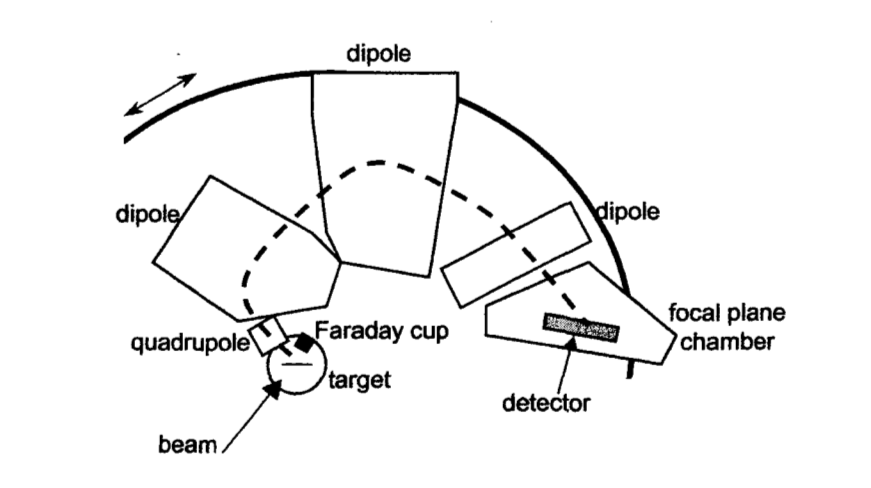
\includegraphics[width=\textwidth]{Q3D_spectrometer.png}
\caption{Schematic of the Q3D magnetic spectrograph at M\"{u}nich used for precision (p,t)/(t,p) spectroscopy \cite{Meyer_thesis}.}
\label{fig:Q3D}
\end{center}
\end{figure}


In the case of a $\Delta$L=0 transition, the angular distribution of detected particles will be extremely forward-peaked; this is an easily observed experimental signature, and is completely unique to $\Delta$L=0, as the measured intensity (differential cross section) can drop by an order of magnitude from $\sim$5$^\circ$ to $\sim$17$^\circ$ \cite{Meyer_pt0_2006}. Confirmation of the J$^\pi$=0$^+$ assignments can be made by comparing the relative cross sections from the experimental data to a Distorted Wave Born Approximation (DWBA) calculation, where an example of this can be seen in Figure \ref{fig:158Gdpt} for the 0$^+$ states in $^{158}$Gd.

\begin{figure}[ht]
\begin{center}
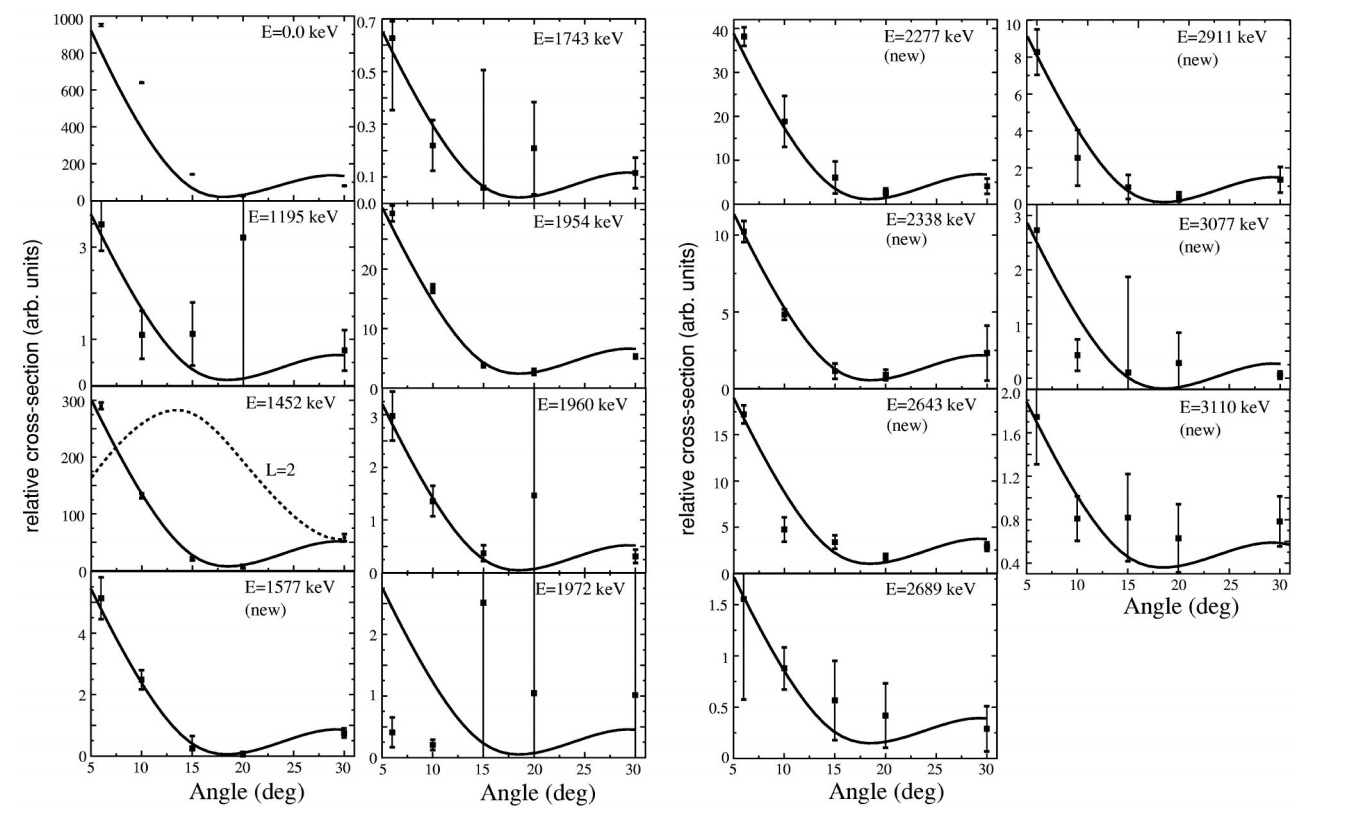
\includegraphics[width=\textwidth]{158Gd(pt).png}
\caption{Angular distribution data for all 0$^+$ states in $^{158}$Gd observed in the (p,t) reaction in \cite{Meyer_pt0_2006}. A DWBA calculation for an L=2 transition is shown as a dotted line in the E=1452~keV plot to show the unique nature of the L=0 transitions (in solid black).}
\label{fig:158Gdpt}
\end{center}
\end{figure}

This renaissance of (p,t)/(t,p) reaction studies has emerged in the past decade, as well as a coordinated flurry of theoretical and experimental efforts and campaigns to begin to answer the still open and important query of the nature of 0$^+$ excitations in the rare-earth region of nuclei \cite{WuAprahamian_multiphonon_1994, Aprahamian2004, Borner_collective1999, Garrett_betavib2001,RevModPhys.83.1467, Bonatsos_collective02009, Clark_pairtransfer2009, Pietrella_beta_2004, Zamfir_doubleoctupole_2002, Sun_0plusnature_PSM_2003}. Figure \ref{fig:Number_0s_Rare_Earth} shows the number of 0$^+$ states for rare earth nuclei, due in large part to the two nucleon transfer reaction studies by Meyer and Lesher \cite{Lesher_158Gdpt,Meyer_pt0_2006}.

\begin{figure}[ht]
\begin{center}
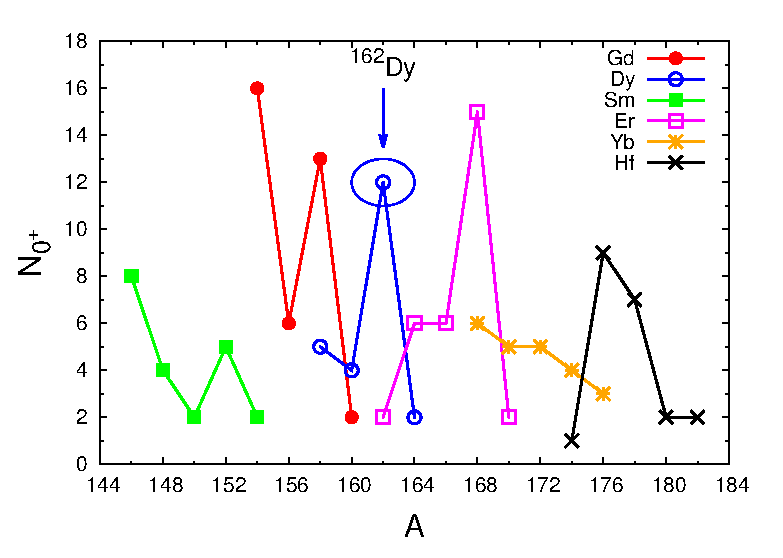
\includegraphics[width=0.95\textwidth]{Gd_Dy_0s_Number.eps}
\end{center}
\caption{Number of 0$^+$ states in rare earth isotopes of Sm, Gd, Dy, Er, Yb, and Hf. $^{162}$Dy is highlighted with a blue circle. \label{fig:Number_0s_Rare_Earth}}
\end{figure}
\newpage
%[MENTION THAT TRANSFER REACTION STRENGTHS TELL US A LITTLE ABOUT 0+ STATES]
In their recent review \cite{RevModPhys.83.1467}, Heyde \& Wood outline several criteria (key experimental fingerprints) to sucessfully elucidate the true nature of these 0$^+$ excitations. 
%, as well as significant proposals to improve the microsopic theories to describe the structure of nuclei far away from shell closures.

\begin{itemize}
\item[I.] Two nucleon transfer reaction strengths, (p,t) or (t,p)
\item[II.] Monopole E0 strengths, $\rho^2$(E0)
\item[III.] Absolute reduced transition probability measurements, B(E2;0$^+_i\rightarrow$2$^+_{g.s.}$)

\end{itemize}

Individually, the experimental quantities listed above cannot fully probe any collective nature of excitations within the nucleus, but in tandem, can uncover much of the mystery of the makeup of nuclear states.

In many cases (due in part to the pioneering (p,t) measurements made by \cite{Lesher_158Gdpt,Meyer_pt0_2006}) throughout the rare-earth region of nuclei, two nucleon transfer reaction strengths are available; the relative cross sections can provide a clue to pairing configurations in nucleons \cite{RevModPhys.83.1467}. This implies that a large relative cross section between two-nucleon transfers will signify a large single- or two-quasiparticle nature of a particular excited state. Historically, inflated two-nucleon transfer reaction cross sections between 0$^+$ states were observed as evidence of rapid shape change of the nucleus \cite{Clark_pairtransfer2009}. Multinucleon transfer reactions also offer a double-pronged attack, in that the spectroscopy can also find/confirm the existence of 0$^+$ excitations, recalling the (p,t) reactions outlined in \S \ref{sec:study_of_0plus}.

Monopole E0 transitions, the $\gamma$-ray forbidden decay of a 0$^+\rightarrow$0$^+$ transition, provide insight into a unique facet of the nuclear structure, as the transition is directly related to the mean-square nuclear radius, and thus, the extent of deformation. The measurement of E0 transitions offers clues to the nature of 0$^+$ states, but these experimental signatures are far from easy to obtain \cite{Heyde_text}. Since a $\gamma$-ray carries \textit{at least} one unit of angular momentum away from the nucleus, and no angular momentum transfer takes place in a 0$^+\rightarrow$0$^+$ transition, the nucleus must decay via internal conversion electrons. The transition probability of an E0 transition differs in form from the traditional $\gamma$-ray reduced transition probability (see \S \ref{sec:redtab}), but is expressed by the monopole strength, the internal conversion electron analogue, $\rho^2$(E0), instead. A similar amount of experimental and theoretical effort is being made in regards to the E0 transitions in rare-earth nuclei \cite{Ilie_E02011}. %Recent studies using the IBA have examined the behavior of E0 transitions in nuclei \cite{Ilie_E02011} at both the limits of the SU(3) symmetry and in the middle of the symmetry triangle, with connections to the collectivity of states discussed.

Finally, the absolute B(E2) transition probabilities (inversely proportional to the lifetime of excited states) are the largest clue to the collectivity of states, as they hold a vital part in testing both the IBA and the geometric collective model. The measurement of excited state lifetimes (as seen in the upcoming \S \ref{sec:why_lifetimes}) are the main focus on this work. 
%Garrett [REF HERE] (among many others) has shown that shape coexistence (similarities of nuclear shapes between states) is prevalent in excited states of $^{154}$Sm and $^{154}$Gd, nuclei close to the N=80 shell closure and not fully deformed shape, as well as the existence of double-phonon excitations in A~110 Cadmium isotopes [REF HERE]. 

Strong octupole shape correlations have been experimentally observed in spherical/transitional nuclei (and recently in neutron-rich $^{144}$Ba) by the observation of strong E3 multipolarity radiation that decays to the ground state \cite{Bucher_Octupole144Ba_2016,Garrett_2009_negShapeCoex}. Similarly, strong quadrupole-octupole coupling has been observed in the form of 2$^+\otimes$3$^-$ coupling in several cases by the observation of K$^\pi$=2$^-\rightarrow$2$^+_\gamma$ transitions \cite{Pascu_octupole_2015,Spiecker_E1strength,Soloviev_QuadHex}. In all of these cases, we see and stress the importance of reduced transition probabilities connecting nuclear states. One experimental observable that points toward any octupole correlation (as a means to measure reflection asymmetry, a signature of octupole deformation) is the measurement of E3-multipolarity radiation, which we do not employ in this work due to the lack of detection of this type of radiation. However, significant (albeit less than straightforward) emphasis is placed in the measurement of E1 radiation to study octupole vibrations in the deformed rare-earth region \cite{Pascu_octupole_2015,Soloviev_QuadHex}. 

%NEED TO TALK ABOUT HOW OCTUPOLE STATES HAVE BEEN STUDIED TOO
%REFERENCE THE DIFFERENT IBA WORKS DONE IN THE RARE-EARTH REGION

% \section{$\gamma$-ray Emission \& the Electromagnetic Interaction}
% For nuclear excitations well below the energy threshold for particle emission (a majority of excited states in nuclei), the preferred method to de-excite the nucleus is via the emission of a $\gamma$-ray. %This is extremely beneficial to the experimentalist in the laboratory, as modern detectors and instrumentation have evolved in such a way to make $\gamma$-ray spectroscopy a straightforward and common practice. 
\section{Assessing Nuclear Structure from Decay Radiation}
%Decay radiation in any form is the basis for nuclear structure phenomena, since any observed radiation must contain information about the configuration of the nucleus as it brings the nucleus from some initial state to a final state.
The detection of electromagnetic $\gamma$ radiation is of great value when studying the structure of the nucleus. Since $\gamma$-decay of the nucleus is one of the dominant methods of de-excitation for states below the energy threshold for particle emission, a link (some quantum mechanical operator) between two quantum states can be made via the electromagnetic Coulomb process. Usually expressed as a matrix element, Equation \ref{eq:matrix_element} is the manifestation of observables from some corresponding operator (in this case, the electromagnetic operator acting on the nuclear eigenfunctions). In the case of electromagnetic decays, the matrix elements of the E2 multipole transition operators remain a key facet of nuclear structure, as the quadrupole electromagnetic operator drives collective quadrupole transitions in nuclei, lending its importance almost immediately. Similarly, the other multipole expansions of the electromagnetic operator (isovector dipole, isoscalar dipole, octupole, etc.) directly link the charge distributions of two nuclear states, such as the E3 operator for octupole shape change.

\begin{equation}\label{eq:matrix_element}
\mathcal{M}_{fi}=\langle\psi_f\vert\mathcal{H}\vert\psi_i\rangle
\end{equation}

When studying excited states in nuclei, measurement of the transition probability (related to the matrix element) becomes the basis for understanding nuclear structure phenomena. 

% \subsection{Why Measure Lifetimes?}
\label{sec:why_lifetimes}
The transition probability ($\mathcal{W}$) for a $\gamma$-decay that de-excites the nucleus from an initial state to a final state can be expressed in terms of the mean lifetime ($\tau$), the average time the nucleus stays in an excited state, or by the half-life (\textit{t$_{1/2}$}). The exact relationship can be seen in Equation \ref{eq:life_halflife}.

\begin{equation}\label{eq:life_halflife}
\mathcal{W}=\frac{1}{\tau}=\frac{\ln2}{t_{1/2}}
\end{equation}

For an excited state with multiple $\gamma$-decay channels, we can expand the total $\mathcal{W}$ as a sum of all transition probabilities weighted by the branching ratio (BR$_i$) and internal conversion coefficient ($\alpha_i$) of each transition (Equation \ref{eq:BR_W}).

\begin{equation}\label{eq:BR_W}
\mathcal{W}=\sum_i\frac{BR_i}{\tau(1+\alpha_i)}
\end{equation}

The number of full mathematical derivations of Fermi's Golden Rule from time-dependent perturbation theory rivals that of Talmi's estimation of 2$^+$ configurations in Samarium-154 ($\sim$3$\times10^{14}$) \cite{Casten_text}. The exhaustive treatment can be seen in much greater detail in various sources (\cite{Wong_text},\cite{Heyde_text},\cite{BlattWeiss_text}), where (in this work) we will start with Fermi's Golden Rule \cite{Wong_text} in Equation \ref{eq:FermisGR}.

\begin{equation}\label{eq:FermisGR}
\mathcal{W}=\frac{2\pi}{\hbar}\vert\langle\psi_f\vert \mathcal{H}_{EM,int}\vert\psi_i\rangle\vert^2\rho(E_\gamma)
\end{equation}

Here, we can see the direct relationship between the nuclear matrix element and $\gamma$-ray energy-dependent density of states ($\rho$(E$_\gamma$)) to the transition probability, $\mathcal{W}$. This square of the matrix element describes the coupling of the nuclear-based interaction Hamiltonian to an external electromagnetic field, which brings the nucleus from some initial state $\vert\psi_i\rangle$ to a final state $\vert\psi_f\rangle$. This transition, for $\gamma$-decay in the nucleus, is represented by the electric or magnetic multipole operator(s) of order $\lambda$, $\mathcal{O}_{\lambda}$. From Wigner-Eckhart theory, we can remove any angular momentum dependence from the full matrix element ($\vert\mathcal{M}_{fi}\vert$=$\langle\psi_f\vert \mathcal{H}_{int}\vert\psi_i\rangle$) to give us the reduced transition probability in Equation \ref{eq:Wig_B}.

\begin{equation}\label{eq:Wig_B}
  B(\pi\lambda;J_i\rightarrow J_f)=\vert \mathcal{M}_{fi}\vert^2=\frac{1}{2J_i+1}\vert\langle J_f\vert\vert \mathcal{O}_{\lambda}\vert\vert J_i\rangle\vert^2
\end{equation}

Performing a multipole (and subsequent series) expansion of $\mathcal{O}_{\lambda}$ into the spherical Bessel functions, spherical harmonics, and the nuclear current density $\mathcal{J}$($\vec{r}$) (Equations \ref{eq:OE_operator} and \ref{eq:OM_operator}) \cite{Wong_text}, we arrive at Equation \ref{eq:W_B}.

%[explain matrix element as electromagnetic operator WONG182]
\begin{align}
  \mathcal{O}_{\lambda\mu}(E\lambda)=-\frac{(2\lambda+1)!!}{c(\lambda+1)k^{\lambda+1}}\mathcal{J}(\vec{r})\cdot\vec{\nabla}\times(\vec{r}\times\vec{\nabla})(j_\lambda(kr)Y_{\lambda\mu}(\theta,\phi))       \label{eq:OE_operator}\\
\mathcal{O}_{\lambda\mu}(M\lambda)=-\frac{(2\lambda+1)!!}{c(\lambda+1)k^{\lambda}}\mathcal{J}(\vec{r})\cdot(\vec{r}\times\vec{\nabla})(j_\lambda(kr)Y_{\lambda\mu}(\theta,\phi))\label{eq:OM_operator}
\end{align}

\begin{equation}\label{eq:W_B}
\mathcal{W}=\frac{8\pi}{\hbar}\frac{(\lambda+1)}{\lambda[(2\lambda+1)!!]^2}\left(\frac{E_\gamma}{\hbar c}\right)^{2\lambda+1}B(\pi\lambda;J_i\rightarrow J_f)
\end{equation}

%\subsection{Importance of Transition Probabilities}
Now, simply recall Equation \ref{eq:BR_W} to make Equation \ref{eq:BE2exp}, an extremely important quantity for nuclear structure studies, as every non-constant quantity can be determined in laboratory experiments. 

\begin{equation}\label{eq:BE2exp}
B(\pi\lambda; J_i \rightarrow J_f)=\frac{\hbar}{8\pi}\mathcal{F}(\pi\lambda)\frac{BR}{\tau (1+\alpha)}\frac{\lambda[(2\lambda+1)!!]^2}{(\lambda+1)}\left(\frac{\hbar c}{E_\gamma}\right)^{2\lambda+1}
\end{equation}

In Equation \ref{eq:BE2exp}, $\mathcal{F}$($\pi\lambda$) is a measure of the mixing from differing multipolarity $\gamma$ radiation; For pure E1, E2, or M1 transitions, this factor collapses to unity, where $\mathcal{F}$($\pi\lambda$) for mixed E2 \& M1 radiation follows the relations in \ref{eq:FE2} \& \ref{eq:FM1}:

\begin{equation}\label{eq:FE2}
\mathcal{F}(E2)=\frac{\delta^2}{1+\delta^2}
\end{equation}
\begin{equation}\label{eq:FM1}
\mathcal{F}(M1)=\frac{1}{1+\delta^2}
\end{equation}

The multipole mixing fraction $\delta$ is an experimentally measured quantity (to be discussed later) as a ratio of the E2/M1 transition strengths.

\subsection{Importance of Transition Probabilities}\label{sec:redtab}
To provide a comparison of the relative collectivity of a transition on a meaningful scale, it is generally prudent to express B($\pi\lambda$) in terms of a Weisskopf estimate. This formulation assumes that only one nucleon is involved in a particular transition \cite{Wong_text}, and is given in Equations \ref{eq:BwE} and \ref{eq:BwM} for electric-type transitions and magnetic-type transitions, respectively.

\begin{equation}\label{eq:BwE}
B(E\lambda)=\frac{0.12^{2\lambda}}{4\pi}\left(\frac{3}{\lambda+3}\right)^2A^\frac{2\lambda}{3}
\end{equation}
\begin{equation}\label{eq:BwM}
B(M\lambda)=0.12^{2\lambda-2}\frac{10}{\pi}\left(\frac{3}{\lambda+3}\right)^2A^\frac{2\lambda-2}{3}
\end{equation}

These `Weissskopf Units' (W.u.) act as a normalization or `yardstick' for collective strength in nuclei, as B($\pi\lambda$)$\gg$1 imply strong collective motion in the nucleus. In the rare-earth region, nuclear collectivity is generally dominated by nuclear rotation, an incredibly collective phenomenon with transition rates upwards of 100+ Weisskopf units! However, from our presvious observations of vibrational phenomena in deformed nuclei, we observe order(s) of magnitude weaker transition strengths for the rare earth nuclei. Weisskopf units are not universally adopted however, with some (especially older) works relying on the natural units of e$^2$b$^\lambda$. Transition probabilities in this work are reported in W.u., but for the purposes of unit conversion, Table \ref{tab:Weisskopf_conversion} shows this conversion for E1, M1, E2, and E3 transition probabilities for both $^{160}$Gd and $^{162}$Dy.

\begin{table}[ht]
\centering
\caption{WEISSKOPF CONVERSIONS FOR $^{160}$GD AND $^{162}$DY \label{tab:Weisskopf_conversion}}

\begin{tabular}{rlcl|r|l}
 & $\pi\lambda$ &&  $^{160}$Gd & $^{162}$Dy \\ \hline\hline
1~mW.u.& E1 & = & 1.90    & 1.91    & e$^2$b\\
1~W.u. & E2 & = & 5.16E-7 & 5.25E-7 & e$^2$b$^2$\\
1~W.u. & E3 & = & 1.52E-9 & 1.56E-9 & e$^2$b$^3$ \\
1~W.u. & M1 & = & 1.79    & 1.79    & $\mu_N^2$ \\
\end{tabular}\\
\vspace{10pt}
\begin{normalsize}
Unit conversion for transition probabilities from Weisskopf units to e$^2$b$^\lambda$ ($\mu_N^2$ for M1s) for $^{160}$Gd and $^{162}$Dy.
\end{normalsize}
\end{table}

To give these transition probabilities context in a vibrational sense, the electric and magnetic multipole operator is proportional to the phonon annihilation operator, $\textit{\textbf{b}}$ in the vibrational model \cite{Wong_text}. This is again, analogous to the classic harmonic oscillator problem in quantum mechanics, where the basis states that make up the eigenfunctions of the phonon creation/destruction operators. Since the matrix element of this annihilation operator and two harmonic oscillator states is $\sqrt N_{phonon}$, the reduced transition probability for a $\gamma$-decay that destroys an N$_{phonon}$ state will be proportional to the number of phonons in the state, N$_{phonon}$, outlined in Equation \ref{eq:phonon_annihil}.

\begin{equation}\label{eq:phonon_annihil}
\mathcal{O}_\lambda\propto\textbf{\textit{b}}_\lambda\rightarrow \langle\psi_f\vert\textbf{\textit{b}}_\lambda\vert\psi_i\rangle=\sqrt N_{phonon}\rightarrow B(\pi\lambda)\propto N_{phonon}
\end{equation}

This fact implies the transition probability for a double phonon vibrational state will be enhanced in relation to the already inflated B(E2) of a single phonon vibration (in W.u.). These high B(E2) values should be a `signature' of collective motion, however, recall that the B(E2) strength is inversely proportional to the energy of the $\gamma$-ray (B(E2)$\propto$E$_\gamma^{-5}$), meaning higher energy transitions will be suppressed in relation to the lower energy transition probabilities. The delicate balance between interband and full de-exciting transitions must be stressed to fully understand the structure of these states. 

Transition probabilities can also be compared to the `Alaga' rules to provide a benchmark of relative transition strength. The Alaga rules imply that the intrinsic matrix elements for two transitions leaving the same level will be identical (an assumption that the parent state is a rotational excitation), so the ratio of their reduced transition probabilities are only dependent on the square of the Clebsch-Gordan coefficients (Equation \ref{eq:Alaga}). As a first-order approximation, these rules agree remarkably well with experimentally measured B(E2) values, especially for the lowest spin members of a rotational band (again, the bulk of this work). 

\begin{equation}\label{eq:Alaga} 
\frac{B(E2;J_i\rightarrow J_f)}{B(E2;J_i\rightarrow J_f^\prime)}=\frac{\langle J_i K_i 2 (\Delta K)\vert J_f K_f\rangle^2}{\langle J_i K_i 2 (\Delta K)\vert J_f^\prime K_f\rangle^2}
\end{equation}

Of course, a limitation behind the Alaga rules is that it only gives relative transition probabilities, where the absolute B(E2) is needed, and also can only be used to compare transition probabilities for multiple decays out of the same parent state. 
%[this is on page 211 Wong]
%TALK ABOUT BE2S in IBA
\section{Decay and Structure Systematics in the 150$<$A$<$180 Region}\label{sec:Structure_systematics}
Throughout all of the assertions in \cite{RevModPhys.83.1467} and a flurry of experimental and theoretical efforts preceeding and succeeding it, the jury is still out on the nature of low-lying excitations in rare-earth nuclei and the evolution of collectivity with nuclear deformation. Globally, the lifetimes presented in this work aim to elucidate some of the mystery behind the systematic behavior (or lack thereof) of quadrupole and octupole vibrations in deformed nuclei. Before the emergence of 0$^+$ studies with the Q3D spectrometer, there were very few known 0$^+$ excitations in literature, and even less with accompanying lifetime measurements! Historically, the 0$^+$ bands are populated far weaker than their 2$^+$ $\gamma$-band cousins, making direct measurement of their lifetimes with techniques like Coulomb Excitation much less straightforward. Many of the lifetime measurements made in this work are new, in an region of nuclei where literature lifetimes (especially lifetimes of 0$^+$ states) are scarce. Figures \ref{fig:SmSystematics}, \ref{fig:GdSystematics}, \ref{fig:DySystematics}, \ref{fig:ErSystematics}, \ref{fig:YbSystematics}, and \ref{fig:HfSystematics} show the even isotopes of rare-earth nuclei throughout varying degrees of deformation (marked by the R$_{\frac{4}{2}}$ value). Each set of level schemes displays the ground state band, excitation energies of the first excited 2$^+$ bandhead, the energies of all excited 0$^+$ states, literature B(E2) values (in W.u.) for any 2$^+$ or 0$^+$ de-excitations, as well as the proton \& neutron pairing gap (2$\Delta_\pi$ in green and 2$\Delta_\nu$ in blue) for each isotope (calculated from Equations \ref{eq:pairing_gapP} and \ref{eq:pairing_gapN} in \cite{Bender_pairing2000} \& \cite{MANG_pairing1965353}).

\subsection{K$^\pi$=0$^+$,2$^+$ Systematics in Samarium, Gadolinium, and Dysprosium Nuclei}
At the low-mass end of the rare-earth region, which includes Sm, Gd, and Dy isotopes, we are presented with a series of rapidly-changing deformations in the nucleus, as well as a sharp drop in collectivity of the 0$^+_2$ bandheads as they decay to the ground state. The paradigms of the $\beta$-vibration seem to be abundant in nuclei like $^{150}$Sm and $^{154,156}$Gd, with distinctly collective decays to the ground state. However, these nuclei are not considered fully deformed (noted by their R$_\frac{4}{2}\leq$3), so their existence as collective vibrations do not answer our question whether or not deformed nuclei can exhibit collective quadrupole vibrations. We also see the same pockets where we lack lifetime information for all 0$^+$ states in the region, notably $^{146}$Sm, $^{154}$Gd, and $^{156,158}$Dy nuclei. Yet again, the collectivity of the 2$^+$ $\gamma$ bands are consistently well-behaved, speaking to the stability of this vibrational excitation. In all cases except $^{158}$Gd, any candidates for the $\beta$-vibration are well below the pairing gaps drawn for each nucleus, and is to be expected; this case of $^{158}$Gd's most collective decay from a 0$^+$ lying above the pairing gap is extremely curious, and unfortunately does not clear up the nature of 0$^+$ bands in deformed nuclei!

\begin{landscape}
\begin{figure}[ht] 
\begin{center}
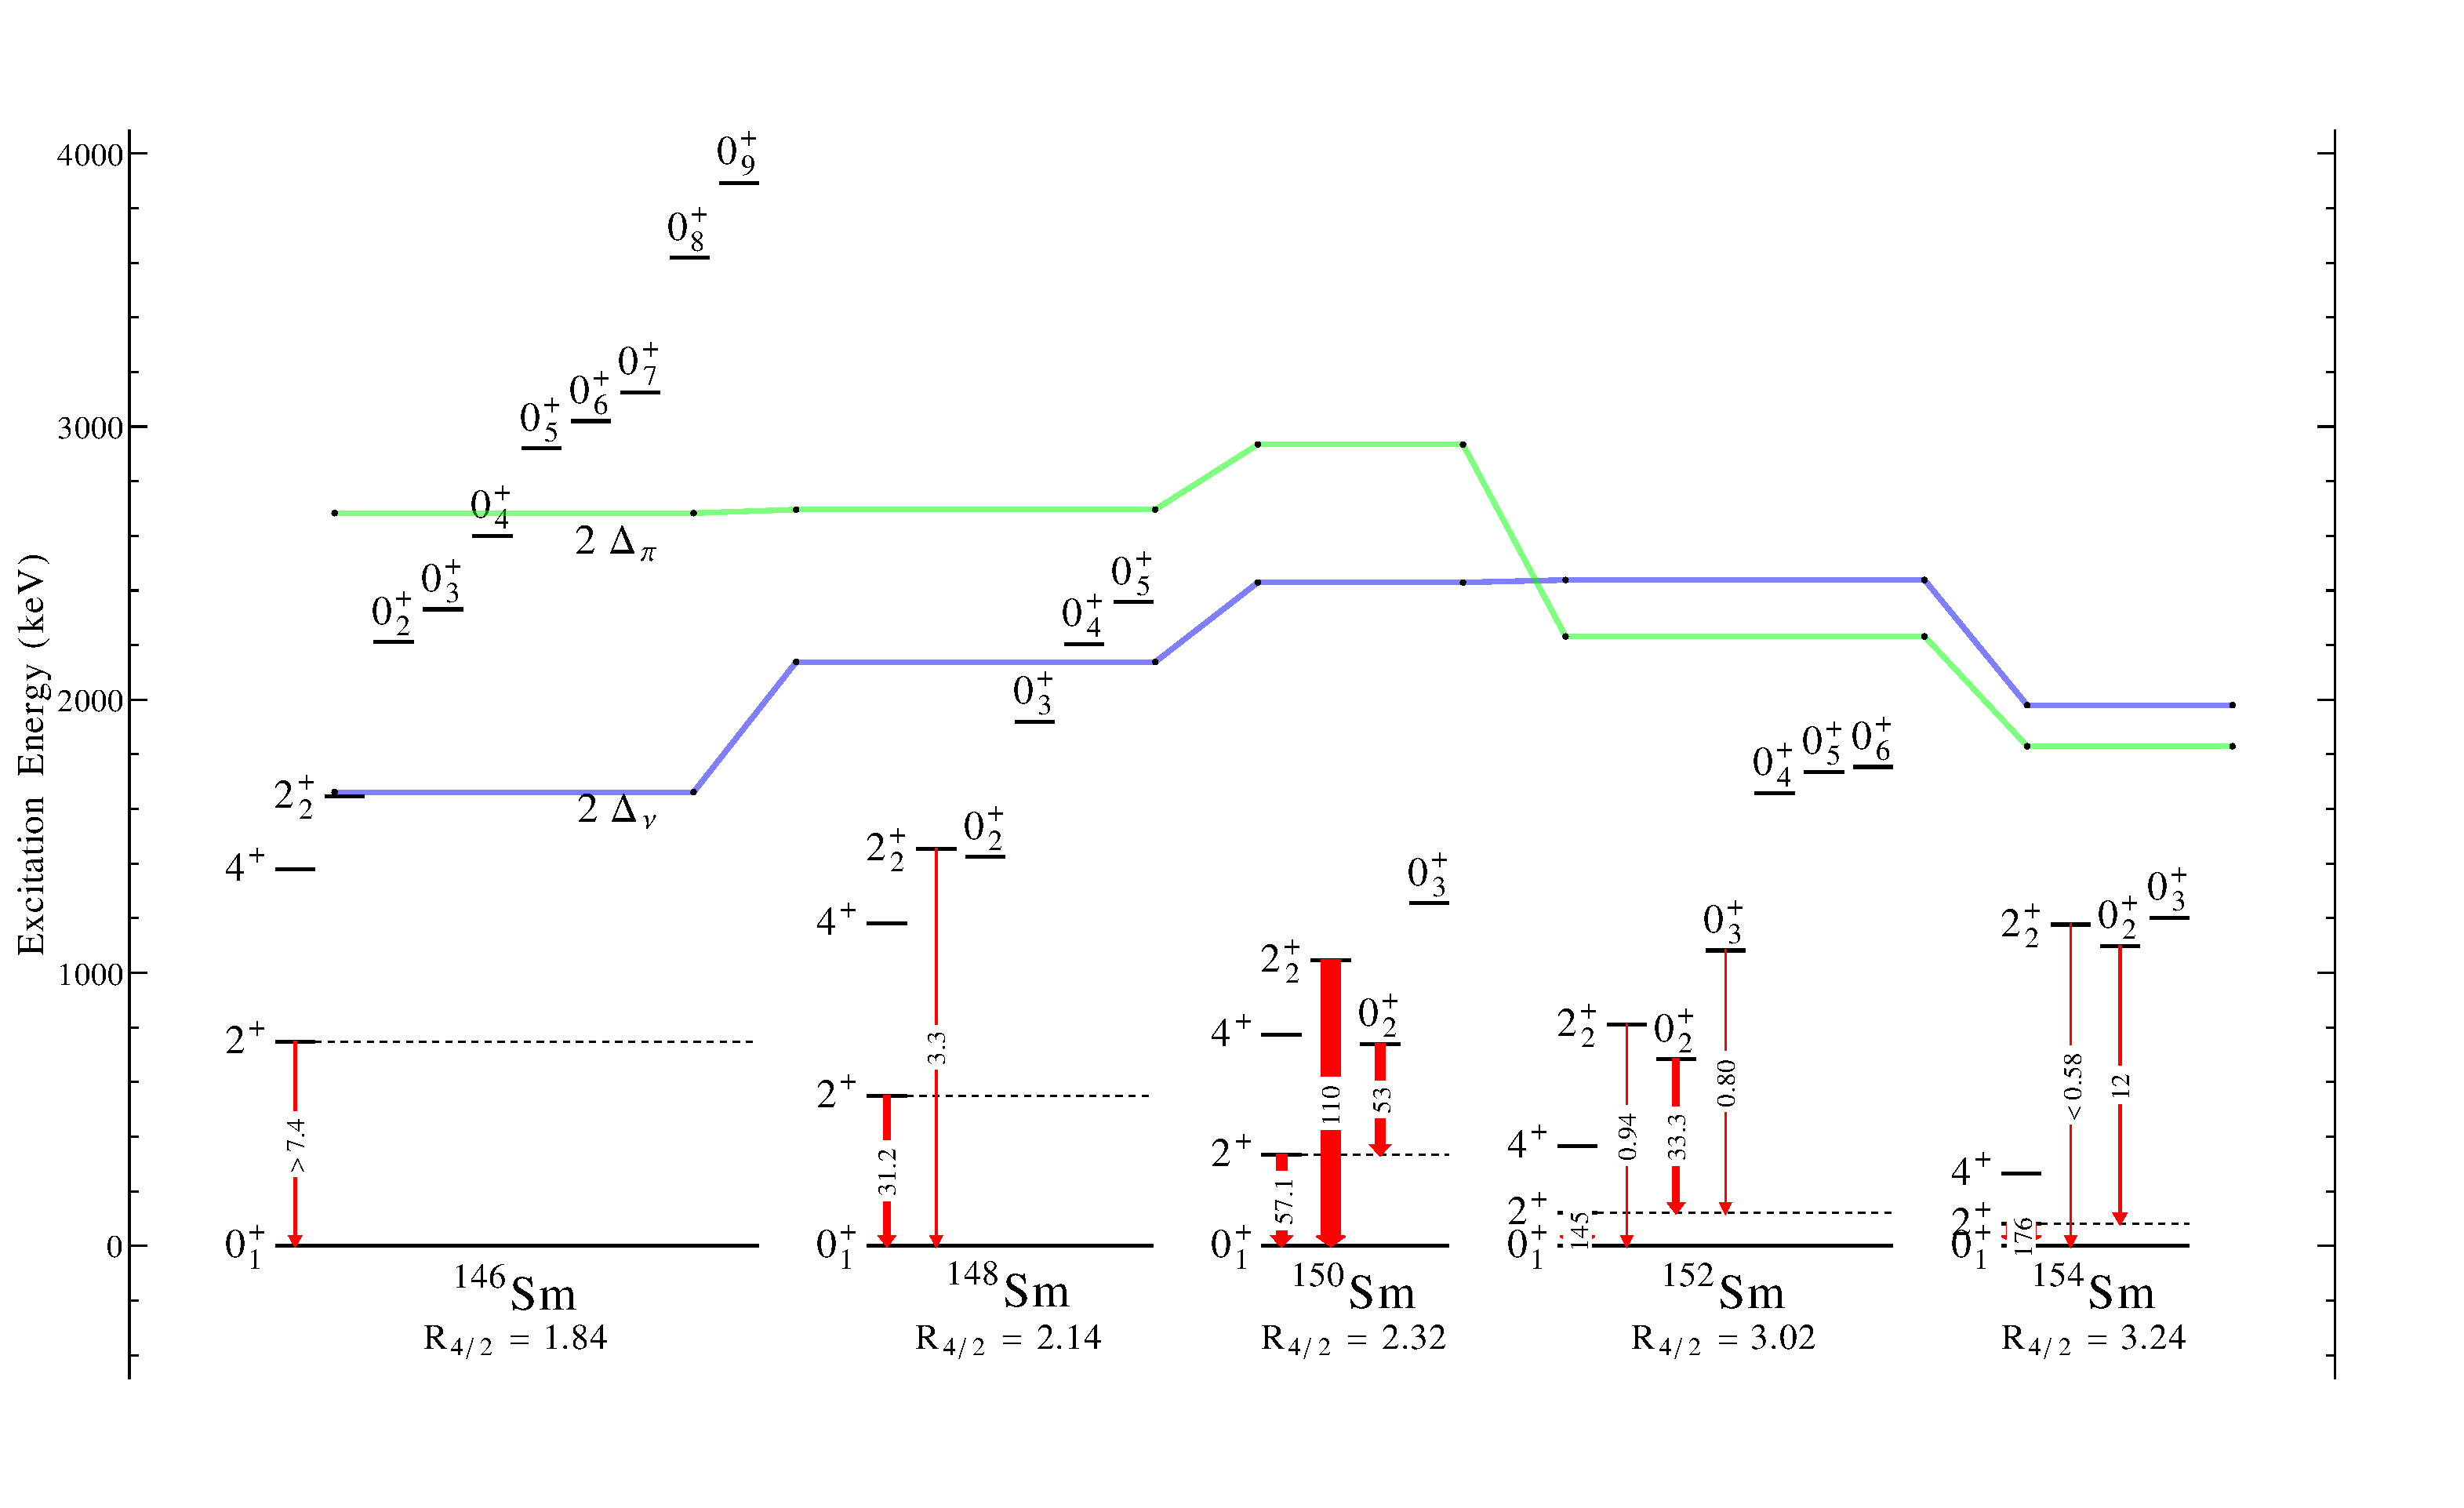
\includegraphics[height=0.8\textheight]{SciDraw_SmSystematics.pdf}
\caption{Systematics for the energies of excited 0$^+$ states, the first excited 2$^+$ bandhead, and low-lying ground state band members for even-even Samarium nuclei. Proton and neutron pairing gaps (2$\Delta_\pi$ and 2$\Delta_\nu$, respectively) are drawn in green and blue and are calculated from Equations \ref{eq:pairing_gapP} and \ref{eq:pairing_gapN}. Transition arrows represent known experimental B(E2) measurements for 0$^+$ bandheads and 2$^+$ bandheads (in W.u. where known).
\label{fig:SmSystematics}}
\end{center}
\end{figure}
\end{landscape}

% \subsection{K$^\pi$=0$^+$,2$^+$ systematics in Gadolinium Nuclei}

\begin{landscape}
\begin{figure}[ht] 
\begin{center}
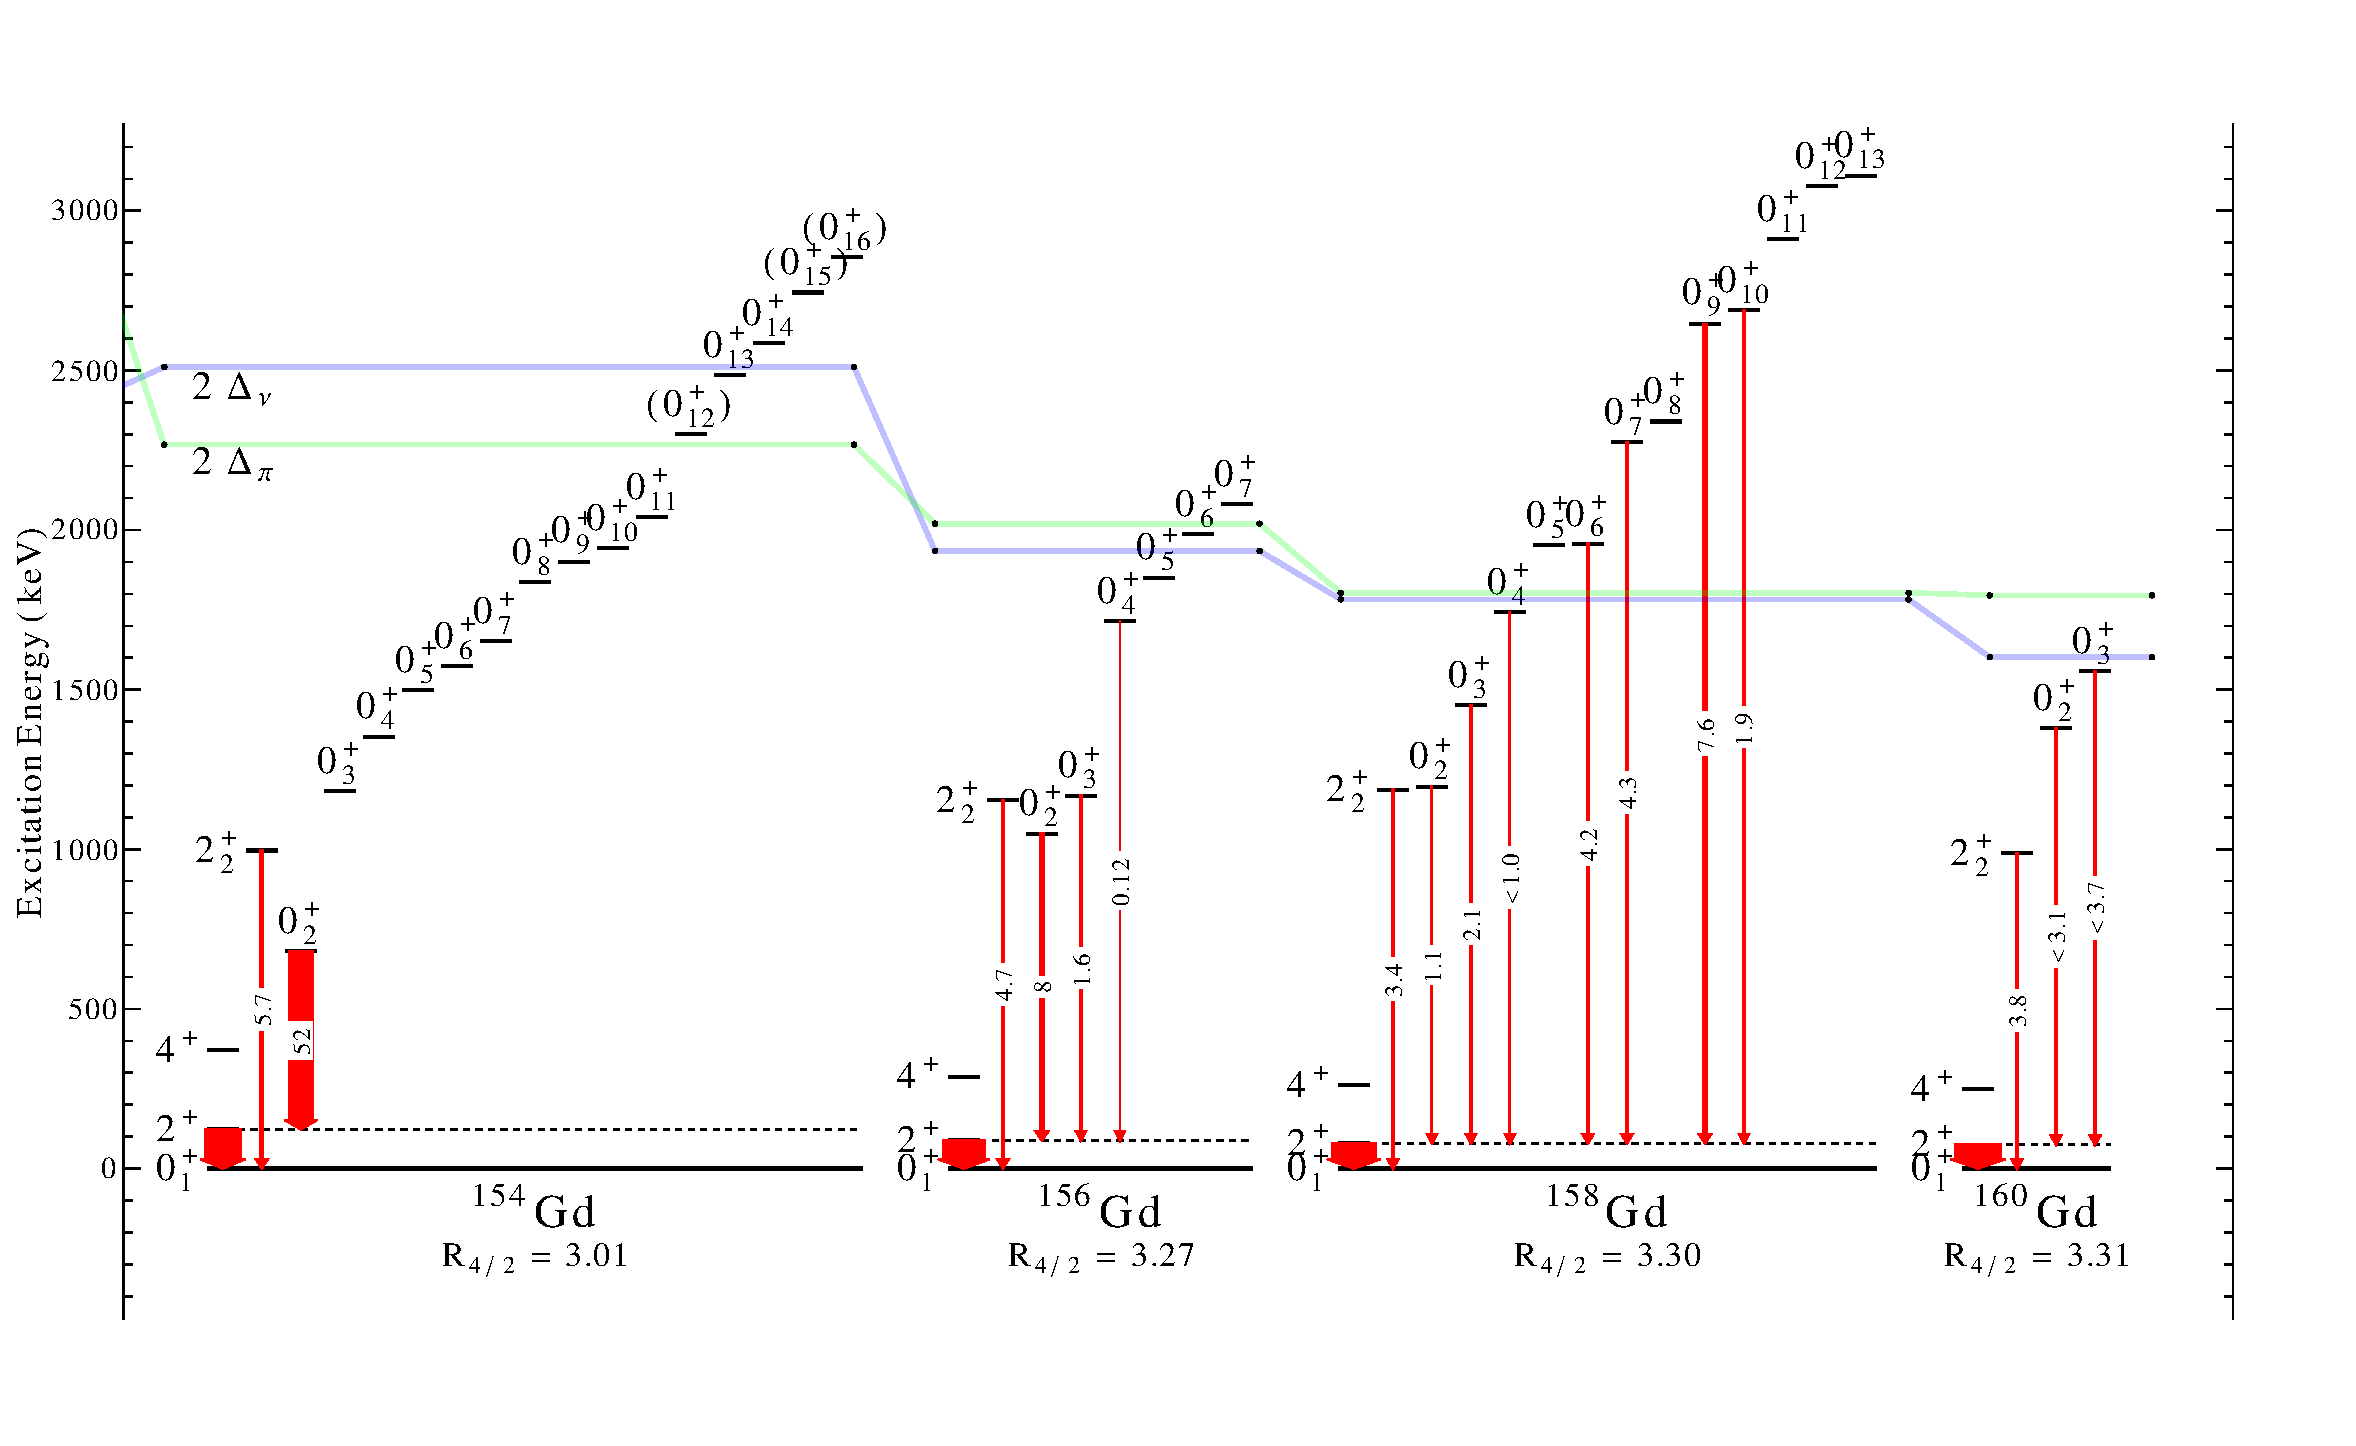
\includegraphics[height=0.8\textheight]{SciDraw_GdSystematics.pdf}
\caption{Systematics for the energies of excited 0$^+$ states, the first excited 2$^+$ bandhead, and low-lying ground state band members for even-even Gadolinium nuclei. Proton and neutron pairing gaps (2$\Delta_\pi$ and 2$\Delta_\nu$, respectively) are drawn in green and blue and are calculated from Equations \ref{eq:pairing_gapP} and \ref{eq:pairing_gapN}. Transition arrows represent known experimental B(E2) measurements for 0$^+$ bandheads and 2$^+$ bandheads (in W.u. where known).
\label{fig:GdSystematics}}
\end{center}
\end{figure}
\end{landscape}

% \subsection{K$^\pi$=0$^+$,2$^+$ systematics in Dysprosium Nuclei}

\begin{landscape}
\begin{figure}[ht] 
\begin{center}
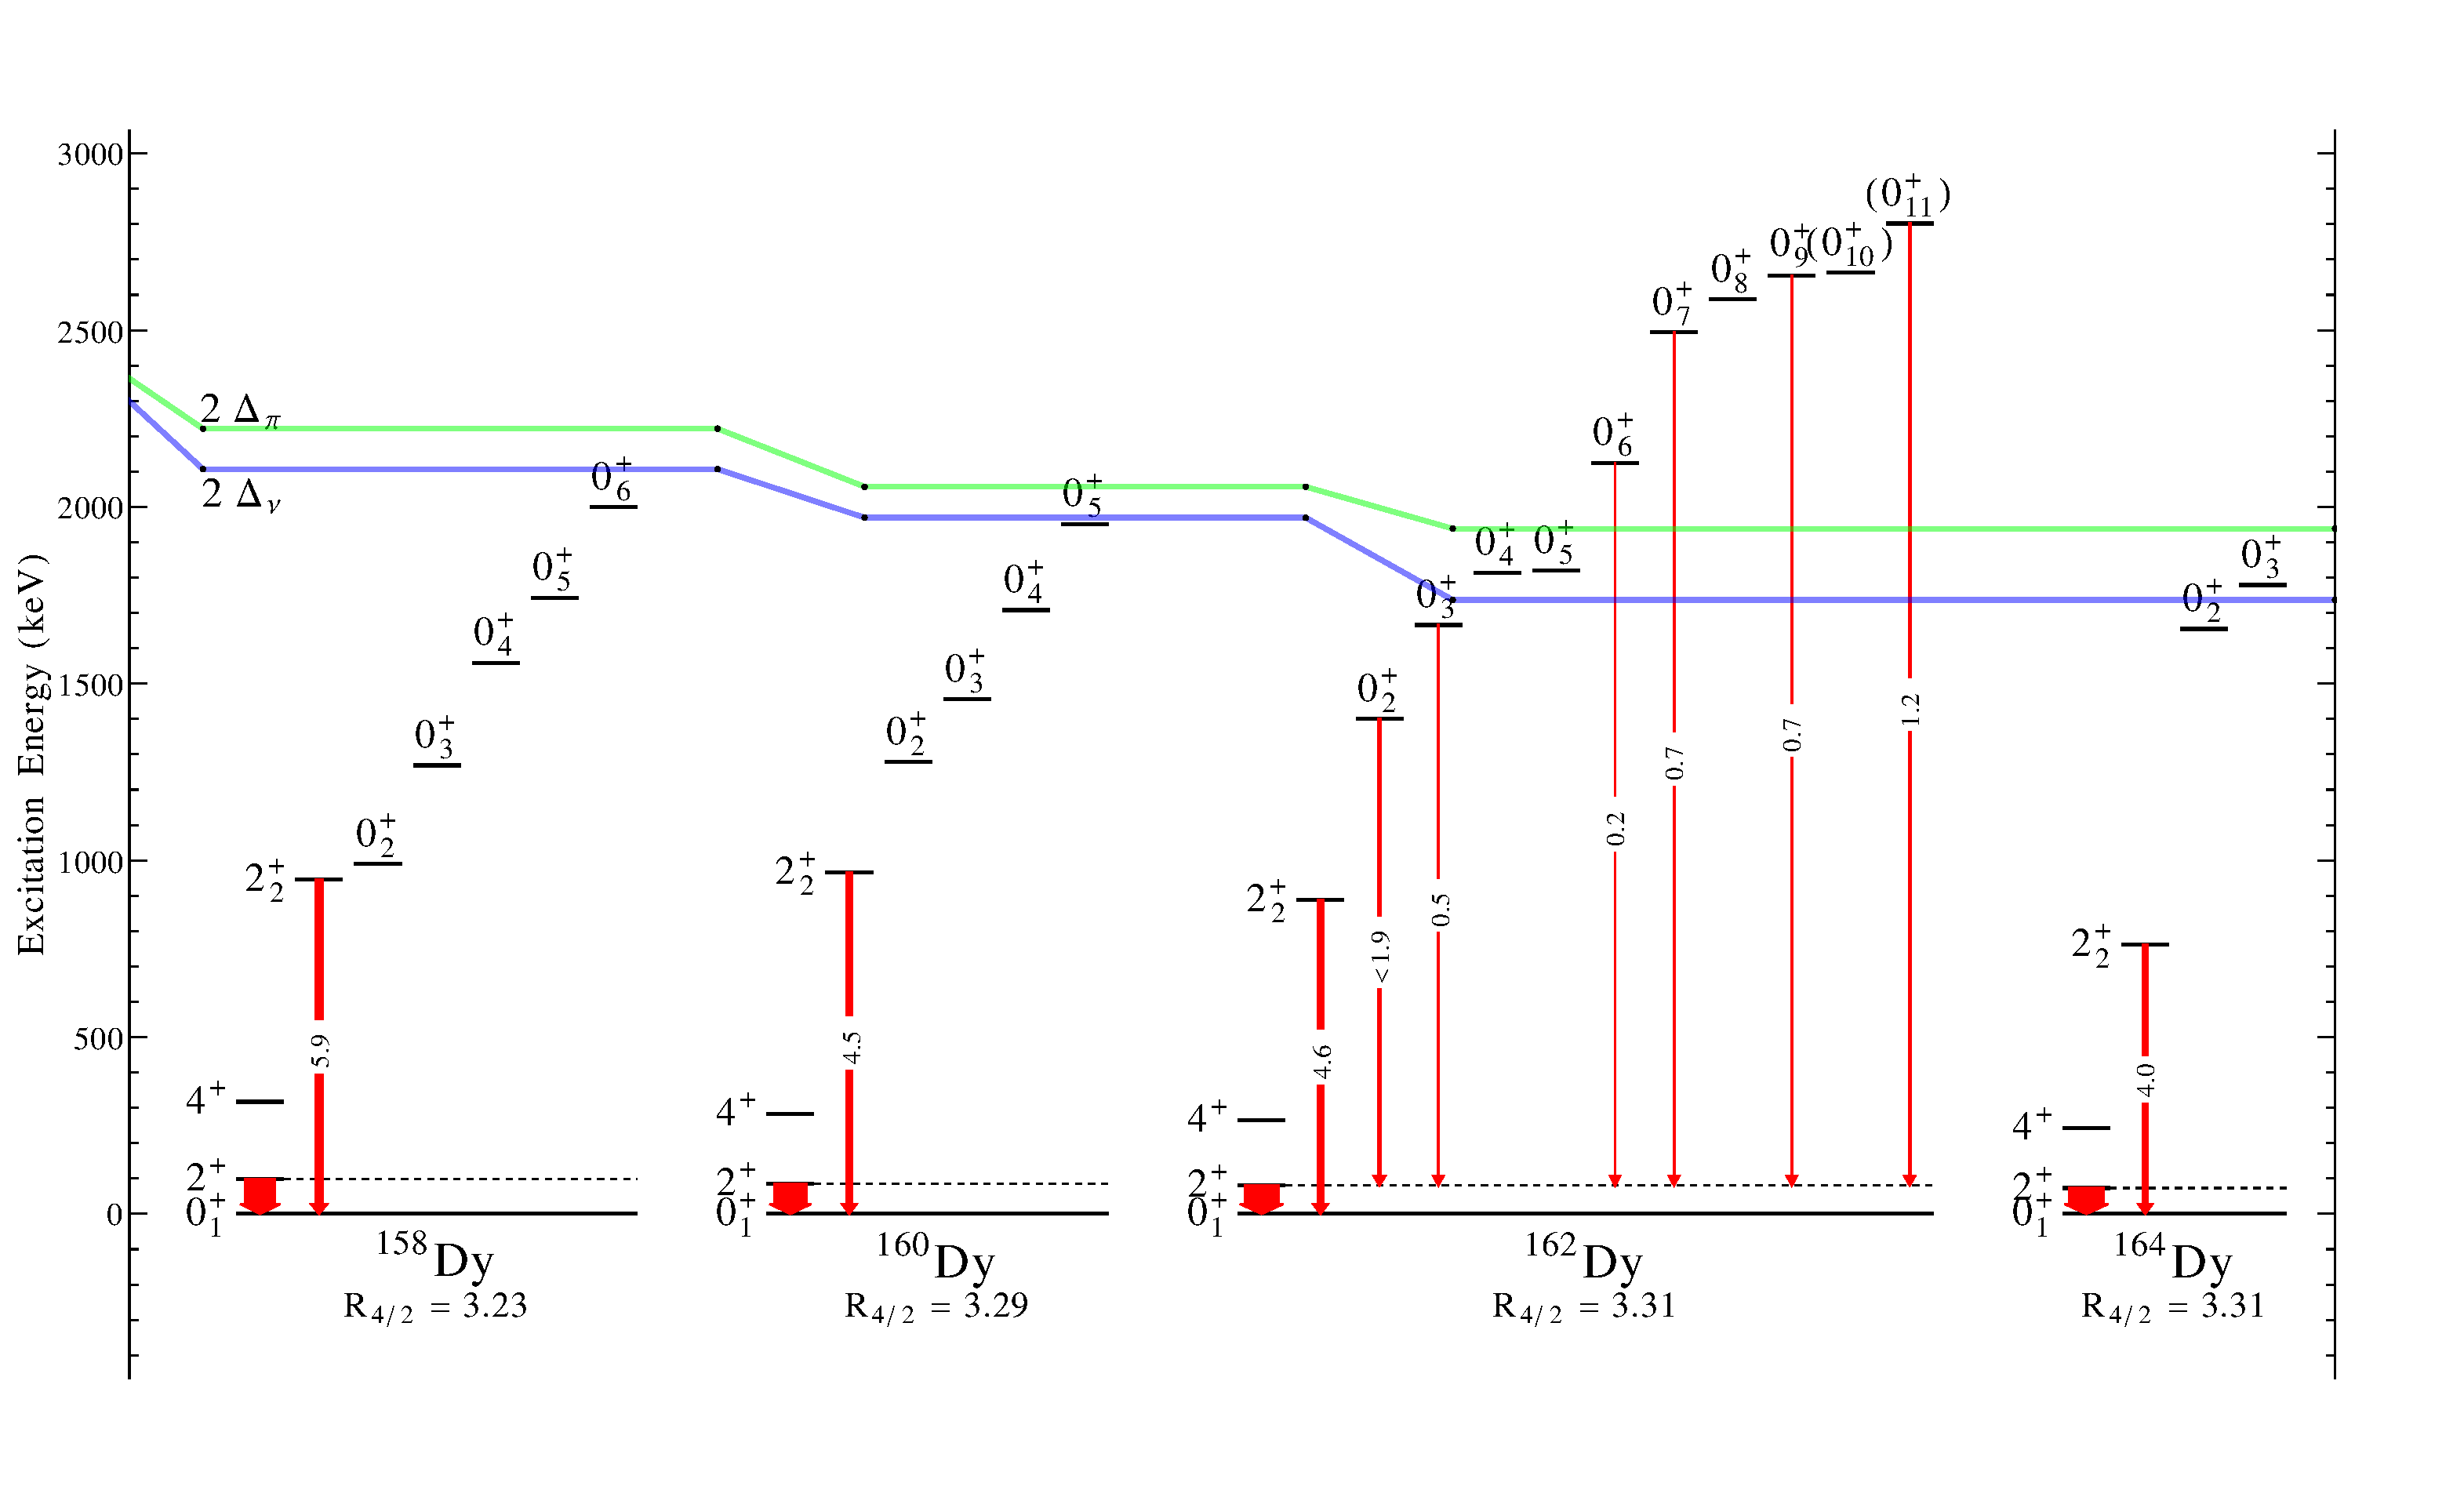
\includegraphics[height=0.8\textheight]{SciDraw_DySystematics.pdf}
\caption{Systematics for the energies of excited 0$^+$ states, the first excited 2$^+$ bandhead, and low-lying ground state band members for even-even Dysprosium nuclei. New transition probabilities are presented in $^{162}$Dy, with the widths proportional to B(E2) values (in W.u.); also shown are the proton and neutron pairing gap (2$\Delta_\pi$ and 2$\Delta_\nu$, respectively) for each isotope.
\label{fig:DySystematics}}
\end{center}
\end{figure}
\end{landscape}

\subsection{K$^\pi$=0$^+$,2$^+$ Systematics in Erbium, Ytterbium, and Hafnium Nuclei}
At the heavier end of the region, we echo some of the same rhetoric as the preceeding nuclei, in that lifetime information for all 0$^+$ states is lacking in select places, but we still retain \textit{some} semblance of the $\beta$-vibration in nuclei like $^{166}$Er and $^{172}$Hf, as well as an overall behavior of the $\gamma$ vibration across the entire chain of isotopes. In contrast, however, these nuclei are all well-deformed, and would be great nuclei to study the feasability of vibrations on top of deformed ground states (take $^{168}$Er for example).

\begin{landscape}
\begin{figure}[ht] 
\begin{center}
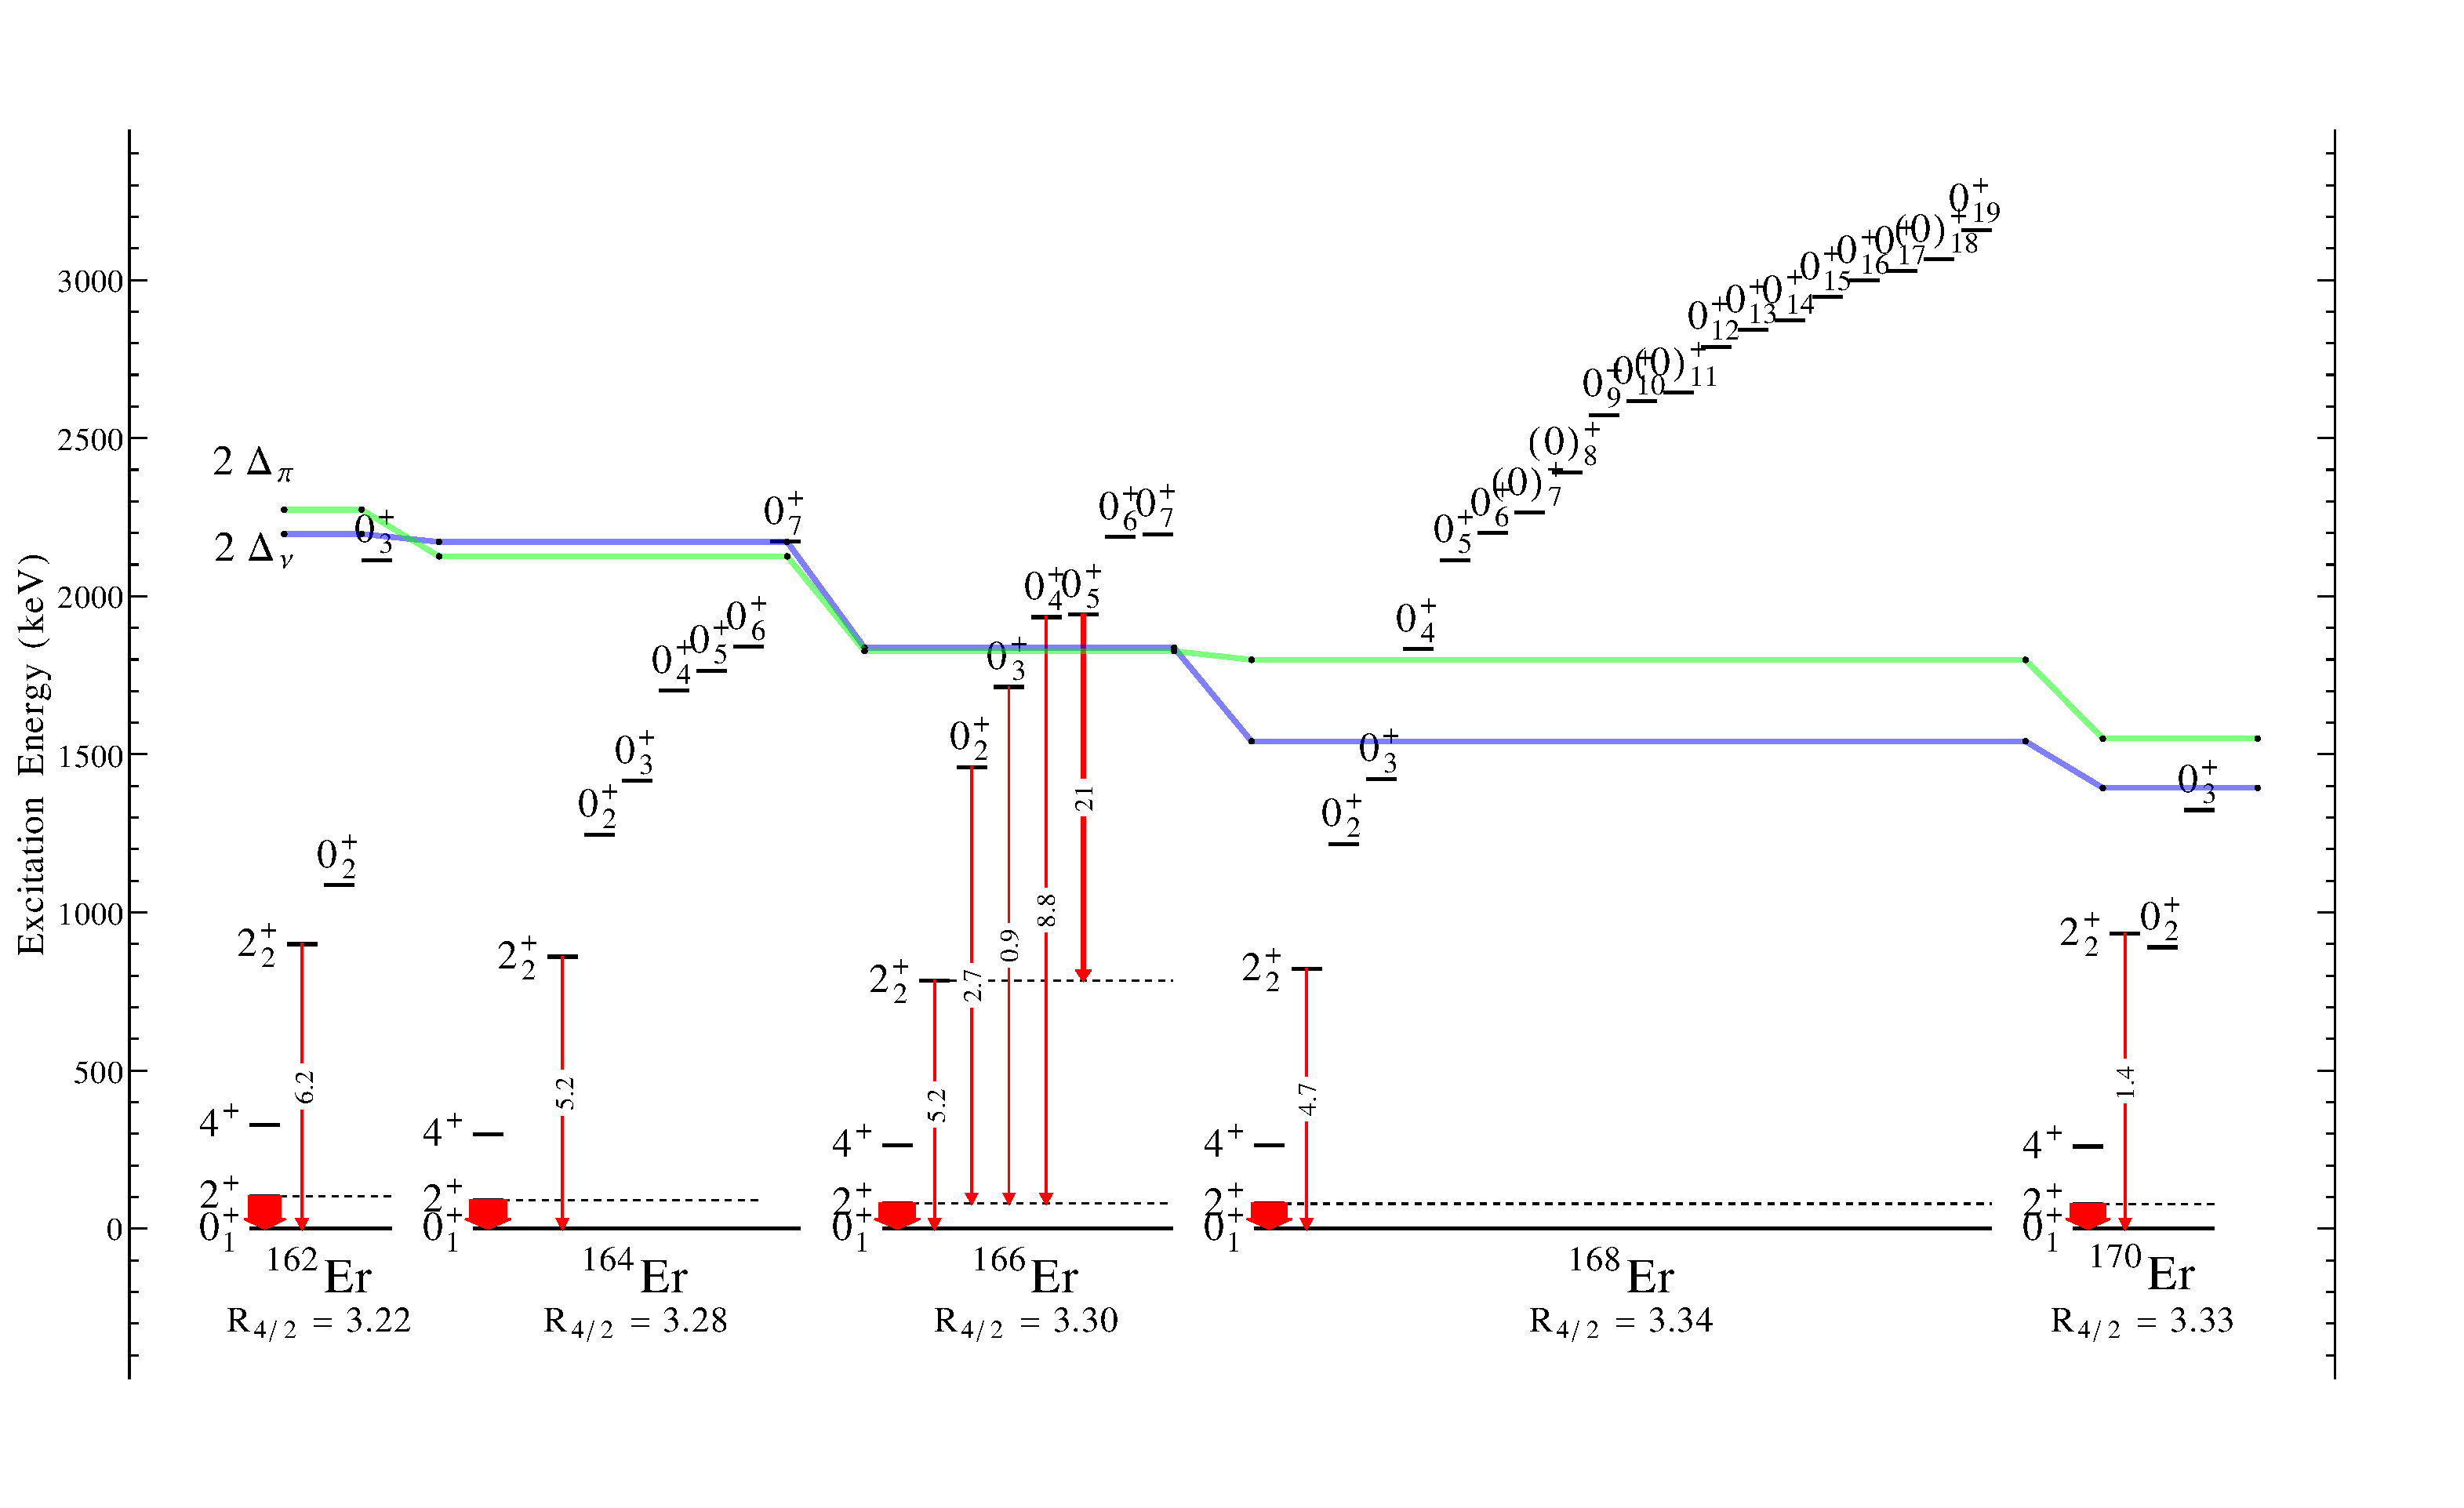
\includegraphics[height=0.8\textheight]{SciDraw_ErSystematics.pdf}
\caption{Systematics for the energies of excited 0$^+$ states, the first excited 2$^+$ bandhead, and low-lying ground state band members for even-even Erbium nuclei. Proton and neutron pairing gaps (2$\Delta_\pi$ and 2$\Delta_\nu$, respectively) are drawn in green and blue and are calculated from Equations \ref{eq:pairing_gapP} and \ref{eq:pairing_gapN}. Transition arrows represent known experimental B(E2) measurements for 0$^+$ bandheads and 2$^+$ bandheads (in W.u. where known).
\label{fig:ErSystematics}}
\end{center}
\end{figure}
\end{landscape}

% \subsection{K$^\pi$=0$^+$,2$^+$ systematics in Ytterbium Nuclei}
\begin{landscape}
\begin{figure}[ht] 
\begin{center}
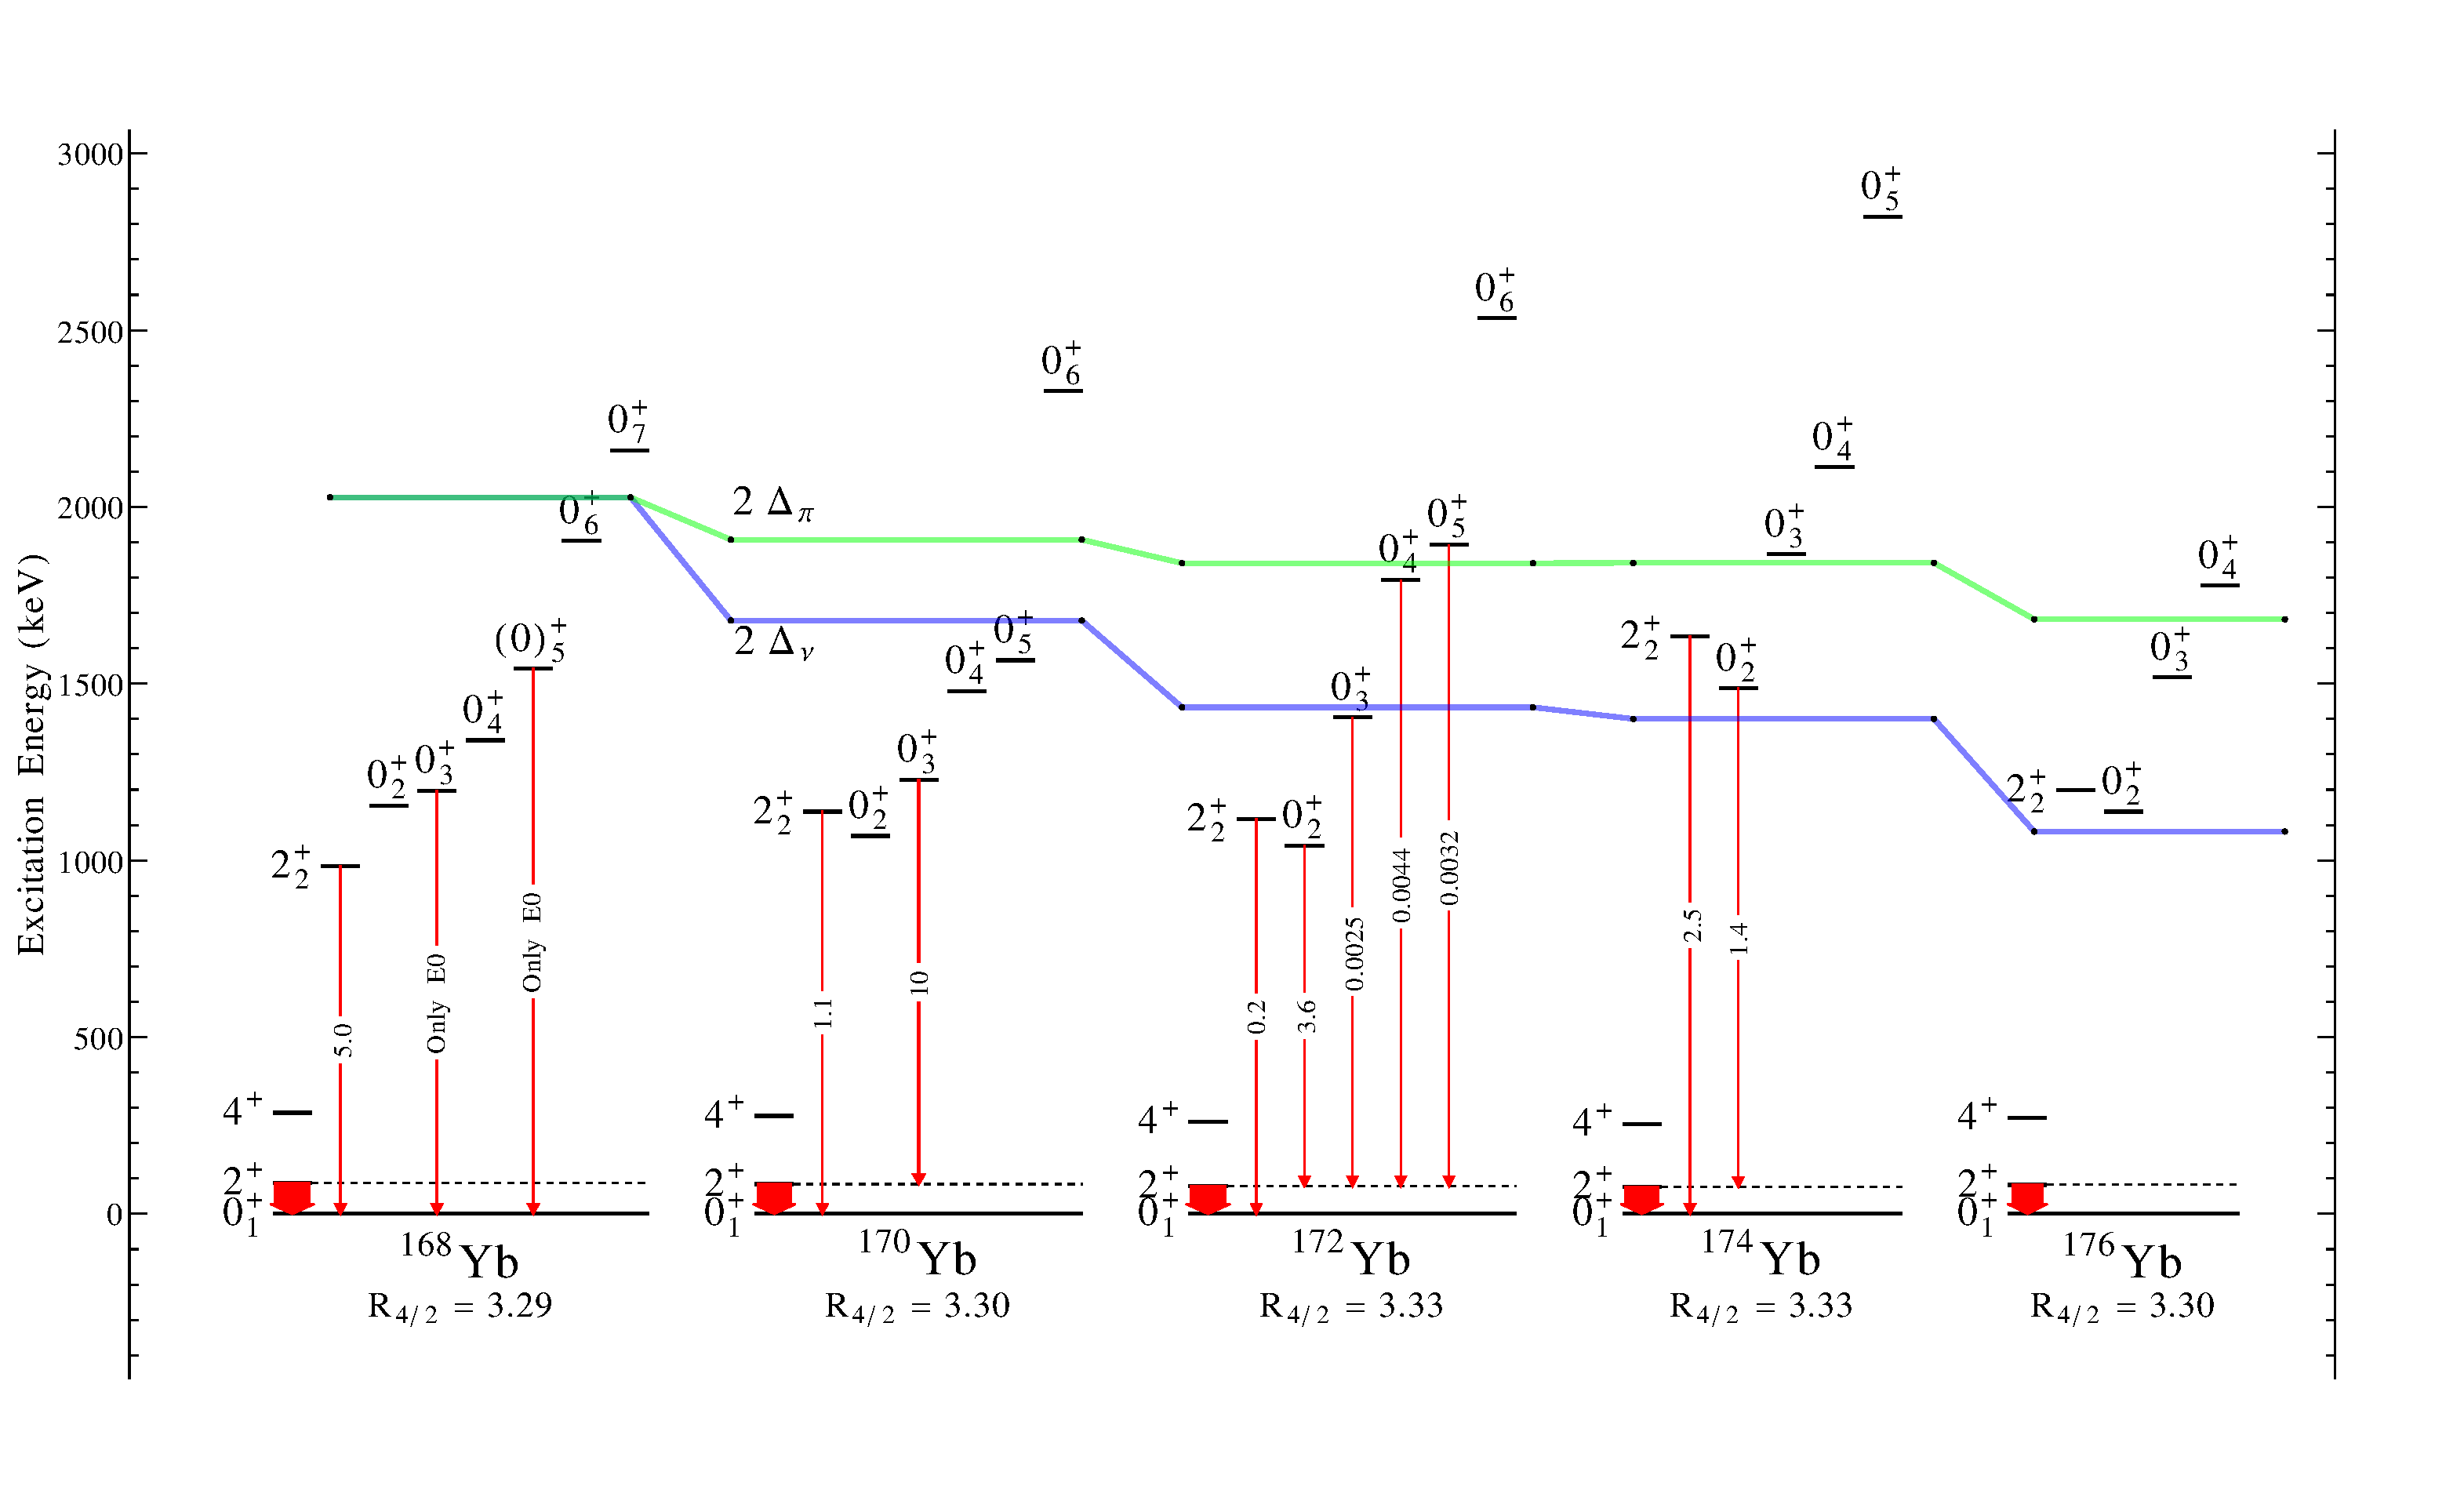
\includegraphics[height=0.8\textheight]{SciDraw_YbSystematics.pdf}
\caption{Systematics for the energies of excited 0$^+$ states, the first excited 2$^+$ bandhead, and low-lying ground state band members for even-even Ytterbium nuclei. Proton and neutron pairing gaps (2$\Delta_\pi$ and 2$\Delta_\nu$, respectively) are drawn in green and blue and are calculated from Equations \ref{eq:pairing_gapP} and \ref{eq:pairing_gapN}. Transition arrows represent known experimental B(E2) measurements for 0$^+$ bandheads and 2$^+$ bandheads (in W.u. where known).
\label{fig:YbSystematics}}
\end{center}
\end{figure}
\end{landscape}
% \subsection{K$^\pi$=0$^+$,2$^+$ systematics in Hafnium Nuclei}

\begin{landscape}
\begin{figure}[ht] 
\begin{center}
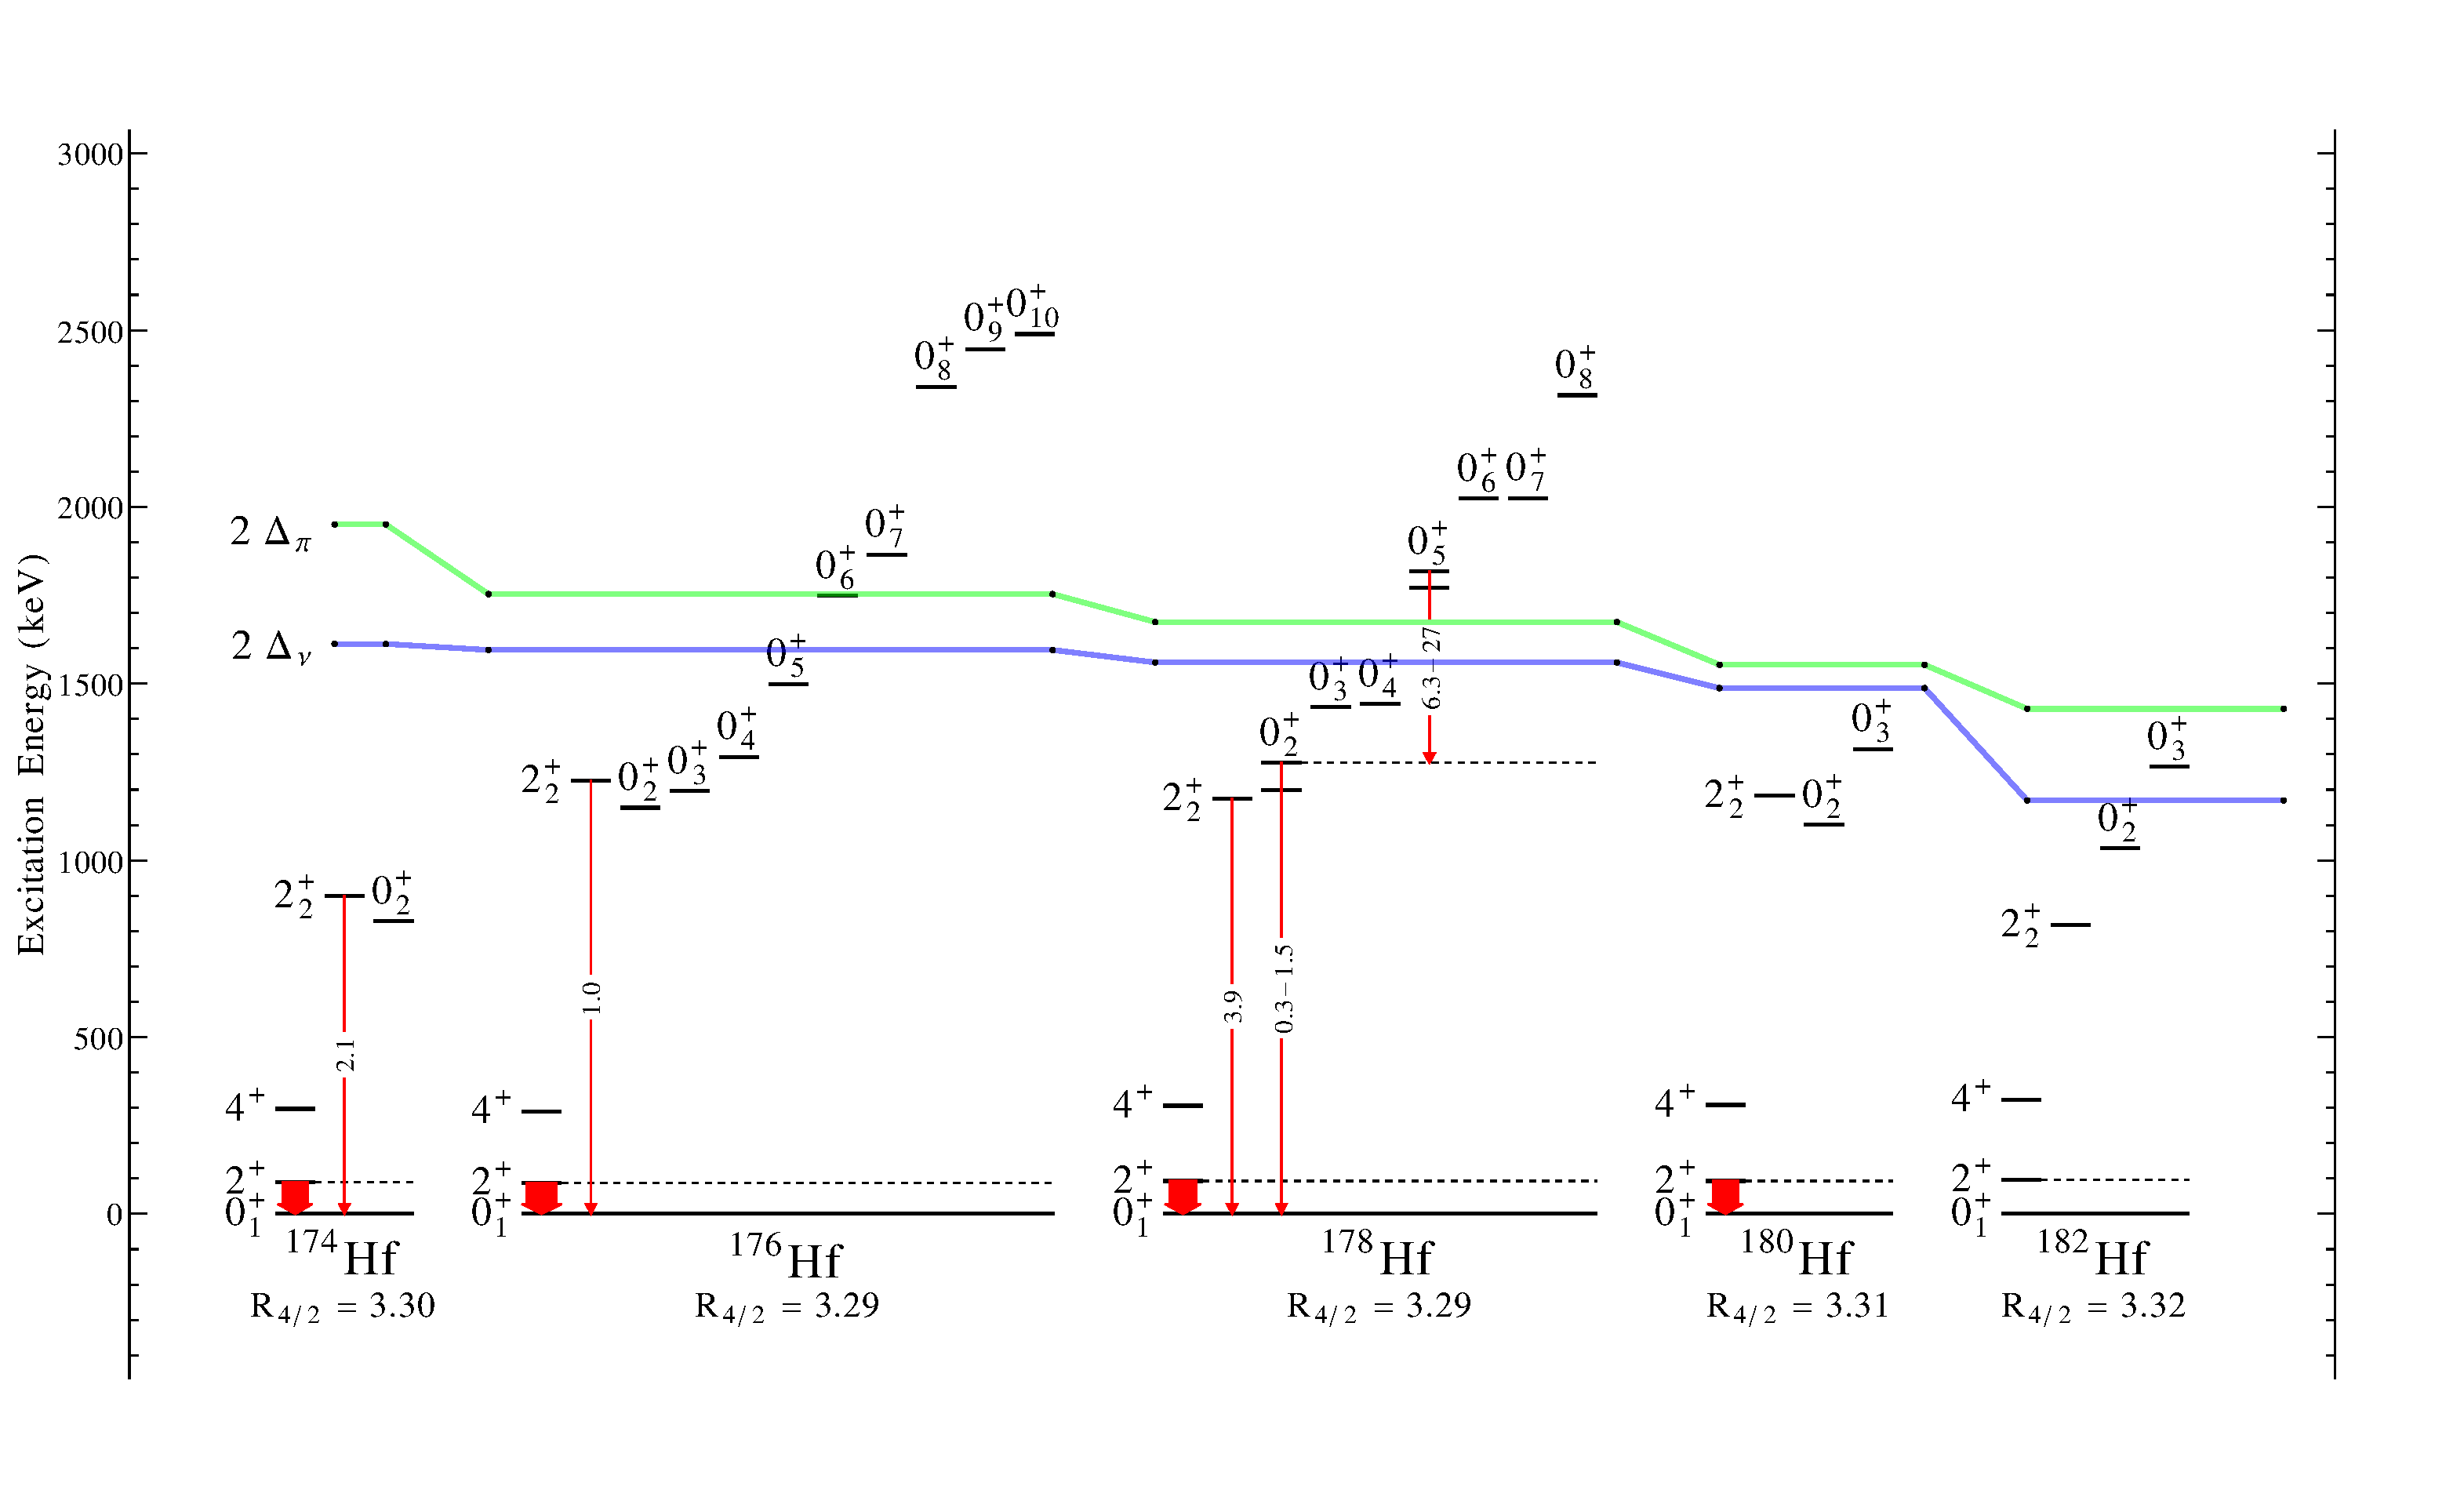
\includegraphics[height=0.8\textheight]{SciDraw_HfSystematics.pdf}
\caption{Systematics for the energies of excited 0$^+$ states, the first excited 2$^+$ bandhead, and low-lying ground state band members for even-even Hafnium nuclei. Proton and neutron pairing gaps (2$\Delta_\pi$ and 2$\Delta_\nu$, respectively) are drawn in green and blue and are calculated from Equations \ref{eq:pairing_gapP} and \ref{eq:pairing_gapN}. Transition arrows represent known experimental B(E2) measurements for 0$^+$ bandheads and 2$^+$ bandheads (in W.u. where known).
\label{fig:HfSystematics}}
\end{center}
\end{figure}
\end{landscape}

In these figures, we can immediately observe some key motivations for performing lifetime measurements in the rare earth region. First, there are currently pockets where we lack literature lifetime information for 0$^+$ excitations in the 150$<$A$<$180 region, especially for states below the proton and neutron pairing gaps, where we would expect to find macroscopic collective motion. Second, in the Gadolinium nuclei, a particular suppression of the collectivity of the lowest-lying 0$^+$ state appears as the static deformation increases. This decrease in collective strength complements the long-standing irregularities in collective strength of 0$^+$ excitations, highlighted by the otherwise `well-behaved' collectivity of the lowest lying K$^\pi$=2$^+$ bands \cite{Casten_0plusbehavior2005, Bonatsos_collective02009}. Lastly, this general inconsistency in collective strength of the 0$^+$ states must be further investigated (previous studies include \cite{Sharpey-Schafer2011,SharpeySchafer_beta2011,Garrett_02_beta}) to match the assertions provided in \cite{RevModPhys.83.1467}. It is entirely reasonable to make the case for strongly collective $\beta$-vibrations in spherical or transitionally deformed nuclei with strong B(E2)s to the ground state 2$^+$, (see $^{150,152}$Sm in Figure \ref{fig:SmSystematics} and $^{154}$Gd in \ref{fig:GdSystematics}) where R$_{\frac{4}{2}}<$3, but as we move to the well-deformed, rotational limit of nuclei, the story definitively changes, and the behavior of the lowest-lying 0$^+$ state changes drastically! Nuclei in the rare-earth region along the line of stability have been hallmarks of spectroscopic knowledge, being some of the most well-studied nuclei for decades, giving us a well-defined goal to characterize the multitude of states where we have a wealth of knowledge as a foundation!

%We also see the various double-phonon cases of 166Er and 178Hf, yet these excitations are only a few in the vast sea of 0+ excitations in rare-earth nuclei. 









\subsection{Negative Parity States in Gadolinium and Dysprosium Nuclei}


We can also see the lack of lifetime information for low-lying negative parity states in rare-earth nuclei, of which, we will study the same cases ($^{160}$Gd and $^{162}$Dy) for the isotopic chains of even-even rare-earth nuclei. Figures \ref{fig:GdSystematics_Octupole} and \ref{fig:DySystematics_Octupole} show the energy systematics for the lowest-lying negative parity bands across isotopes. Immediately again, we see the enegies of the negative parity states mentioned in \S \ref{sec:excitedstates} in regards to the shifting and re-ordering of the split negative parity bands. Again, just like the K$^\pi$=0$^+$ bands, crucial lifetime information for these states is scarce (only 6 lifetimes of negative parity states are known in Dysprosium nuclei); given the number of excitations below the pairing gap (where we expect to see collective excitations), measurement of the B(E1) transition probabilities can allude to any octupole correlations as a phonon excitation in the nuclei discussed in this work, yet the most important piece of experimental evidence (which still remains out of the scope of the experiments performed in this work) is the absolute B(E3) transition probabilities linking states. Enhanced B(E1) strengths have been attributed to the octupole vibration as a type of reflection asymmetry, but are not a smoking gun of the octupole vibration, but more and more nuclei in the rare-earth region display an enhanced degree of dipole strength in the octupole vibration \cite{Soloviev_QuadHex,Pascu_octupole_2015}. 

\begin{landscape}
\begin{figure}[ht] 
\begin{center}
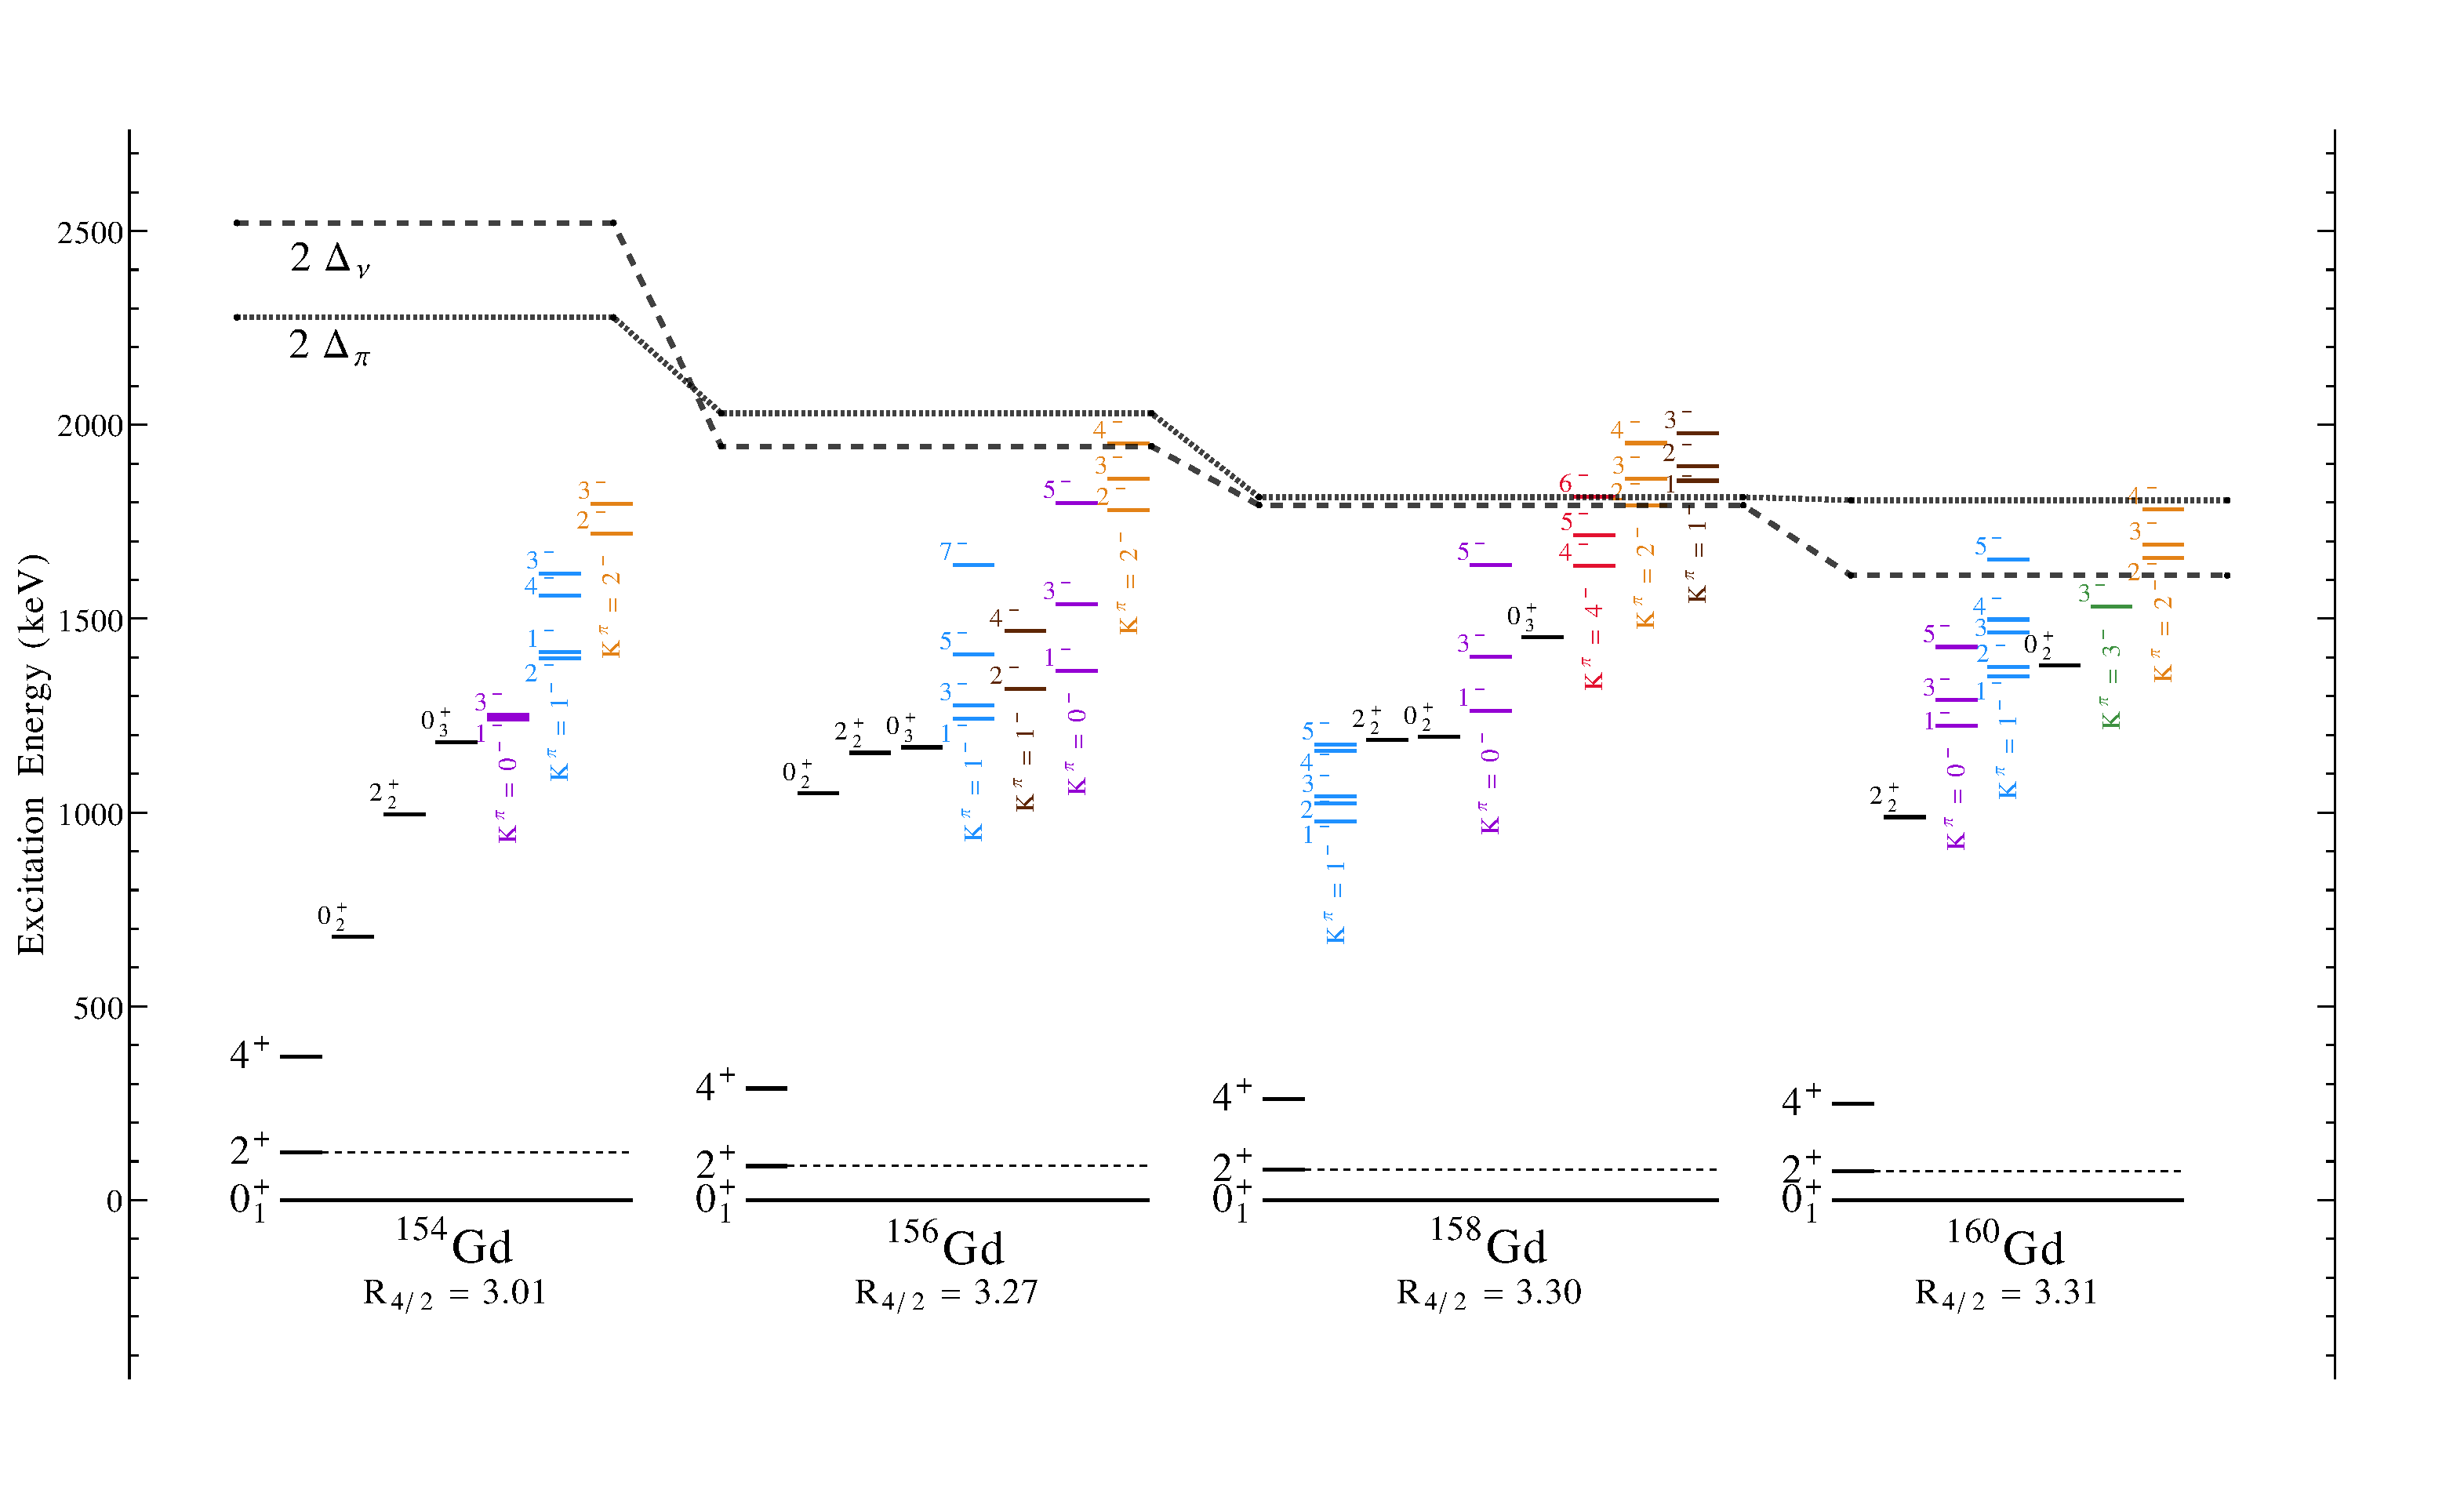
\includegraphics[height=0.8\textheight]{SciDraw_Gd_Octupole_Systematics_FULL.pdf}
\caption{Systematics for the energies of excited negative parity states, the first excited 2$^+$ bandhead, and low-lying excited 0$^+$ states below the pairing gap (2$\Delta_\pi$ and 2$\Delta_\nu$) for even-even Gadolinium nuclei.}
\label{fig:GdSystematics_Octupole}
\end{center}
\end{figure}
\end{landscape}

\begin{landscape}
\begin{figure}[ht] 
\begin{center}
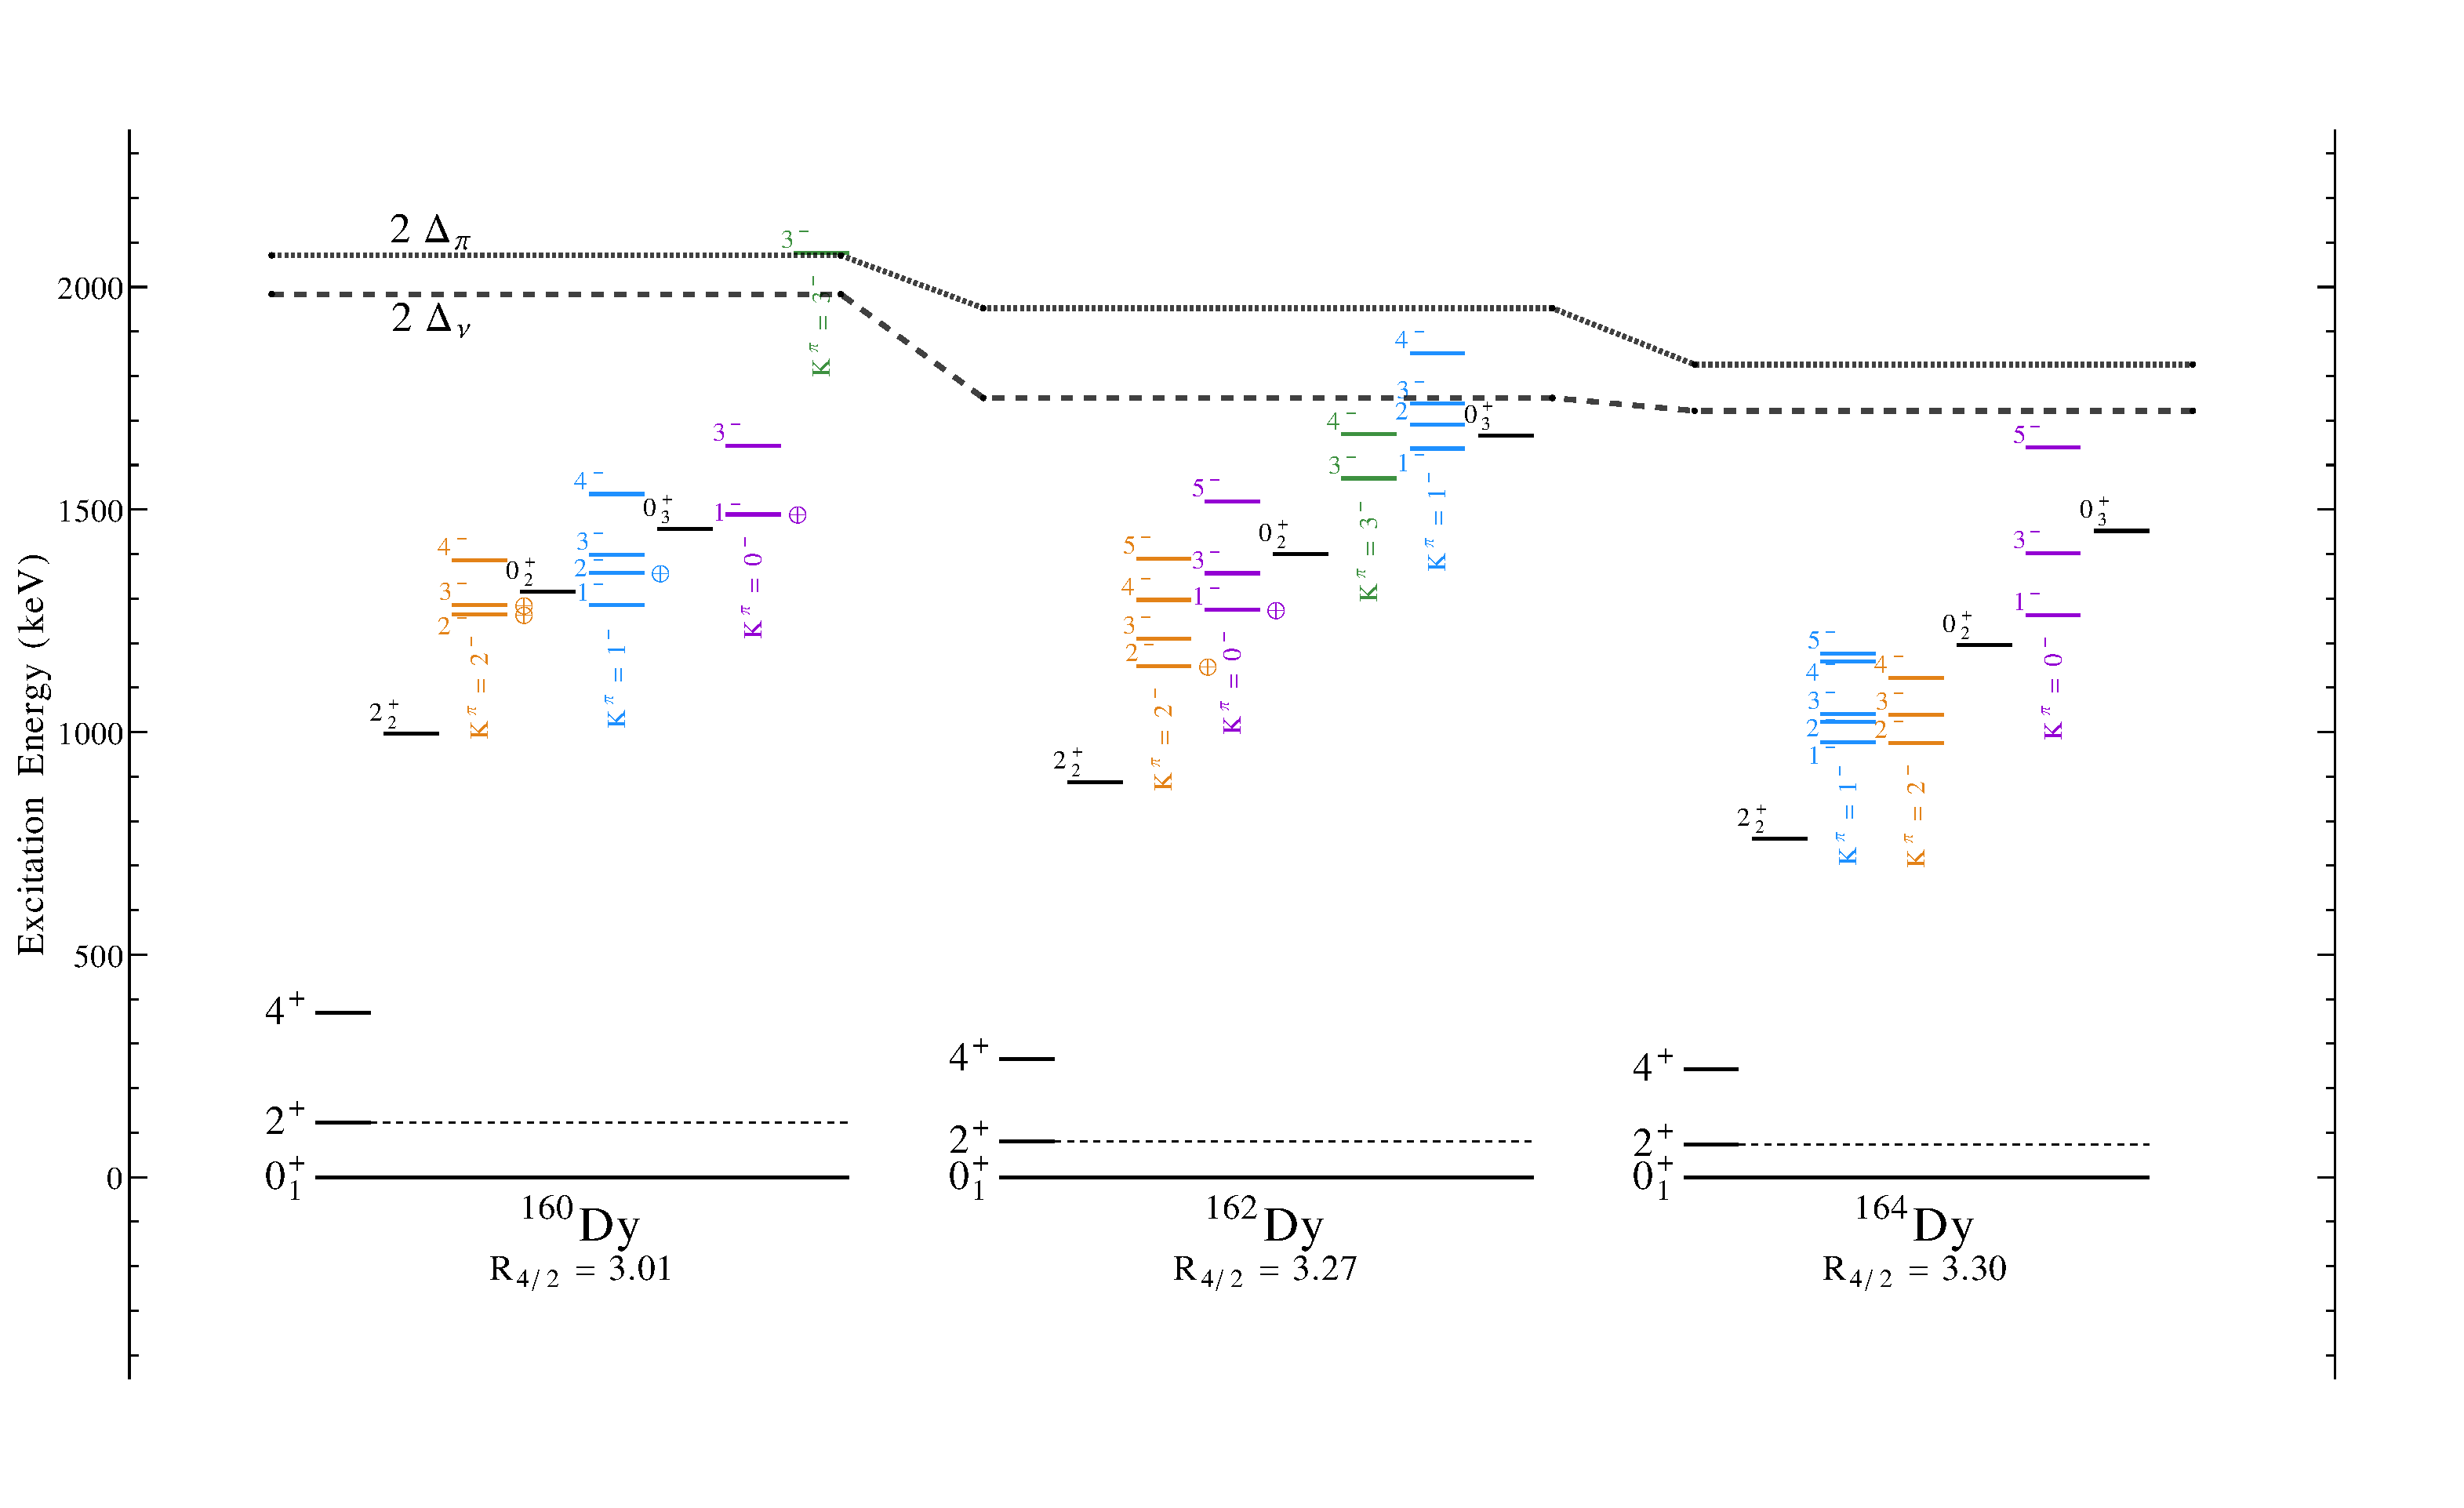
\includegraphics[height=0.8\textheight]{SciDraw_DySystematics_Octupole.pdf}
\caption{Systematics for the energies of excited negative parity states, the first excited 2$^+$ bandhead, and low-lying excited 0$^+$ states below the pairing gap (2$\Delta_\pi$ and 2$\Delta_\nu$) for even-even Dysprosium nuclei. States with a `$\oplus$' marker indicate where a literature lifetime measurement exists.}
\label{fig:DySystematics_Octupole}
\end{center}
\end{figure}
\end{landscape}

\subsection{Multiphonon Configurations in Deformed Nuclei}

We end discussion of the systematics of rare-earth nuclei with any known multiphonon configurations (K$^\pi$=0$^+$,4$^+$ $\gamma\gamma$ type, K$^\pi$=0$^+$ $\beta\beta$). Figure \ref{fig:RareEarth_Multiphonon} contains a series of level schemes of rare-earth nuclei with measured and confirmed two-phonon states; these states are evident by the observation of collective decays to known collective states. For example, the 4$^+$ $\gamma\gamma$-vibration in $^{166}$Er decays via a 7.4~Weisskopf unit B(E2) to the bandhead of the 2$^+$ $\gamma$-vibration (it then subsequently decays via a collective B(E2) to the ground state). As with previous assertions about the `reliability' of the $\gamma$-vibration as a paradigm of nuclear collective vibrations, Figure \ref{fig:Rare_Earth_2g_BE2} shows the absolute  B(E2;2$^+_\gamma\rightarrow$0$^+_{gs}$) measurements in the literature from the K$^\pi$=2$^+$ bandheads, simply to highlight its uniformity over the entire deformed rare-earth region. The trend for Samarium nuclei is drastic, but these isotopes lie in a region of extremely fast shape-change, from nearly spherical to fully deformed within a few nucleons! In a perplexing change of rhetoric in the rare-earths, we observe (and continue to investigate) that many well-deformed nuclei do not exhibit the traditional Bohr-Mottelson behavior of a collective $\beta$-vibration existing as the lowest-lying 0$^+$ state. Instead, many of these lowest-lying 0$^+$ states exist as the $\gamma\gamma$-vibration, with distinctly collective transitions to the 2$^+$ $\gamma$-band. Truly, whether or not the notion of a traditional $\beta$-type vibration is valid seems to be lacking in the deformed case, from the current experimental data. Compare the number of known 0$^+$ $\gamma\gamma$ configurations to the preceeding Figures (\ref{fig:SmSystematics,fig:GdSystematics,fig:DySystematics,fig:ErSystematics,fig:YbSystematics,fig:HfSystematics}) that highlight the status of lifetime measurements of the states and we observe the distinct lack of structure information that still plagues the rare-earth region. No known $\beta\gamma$-vibrations have been observed in the rare-earth nuclei at any excitation energy via a collective transition to a collective $\beta$ or $\gamma$-vibration. However, the 0$^+_5$ state in $^{178}$Hf \textit{could} be the first experimental evidence of a $\beta\beta$ vibration, pending the confirmation of the 0$^+$ state as a collective $\beta$-vibration; as it stands now, the collectivity of the $\beta$-band is tentative, ranging from non-collective to a distinct level of collectivity. If the lowest 0$^+$ band in $^{178}$Hf is indeed a collective $\beta$-vibration, we already have the experimental evidence of a collective transition from another K$^\pi$=0$^+$ band built on top of it, making the 0$^+_5$ band a $\beta\beta$-vibration.

\begin{landscape}
\begin{figure}[ht] 
\begin{center}
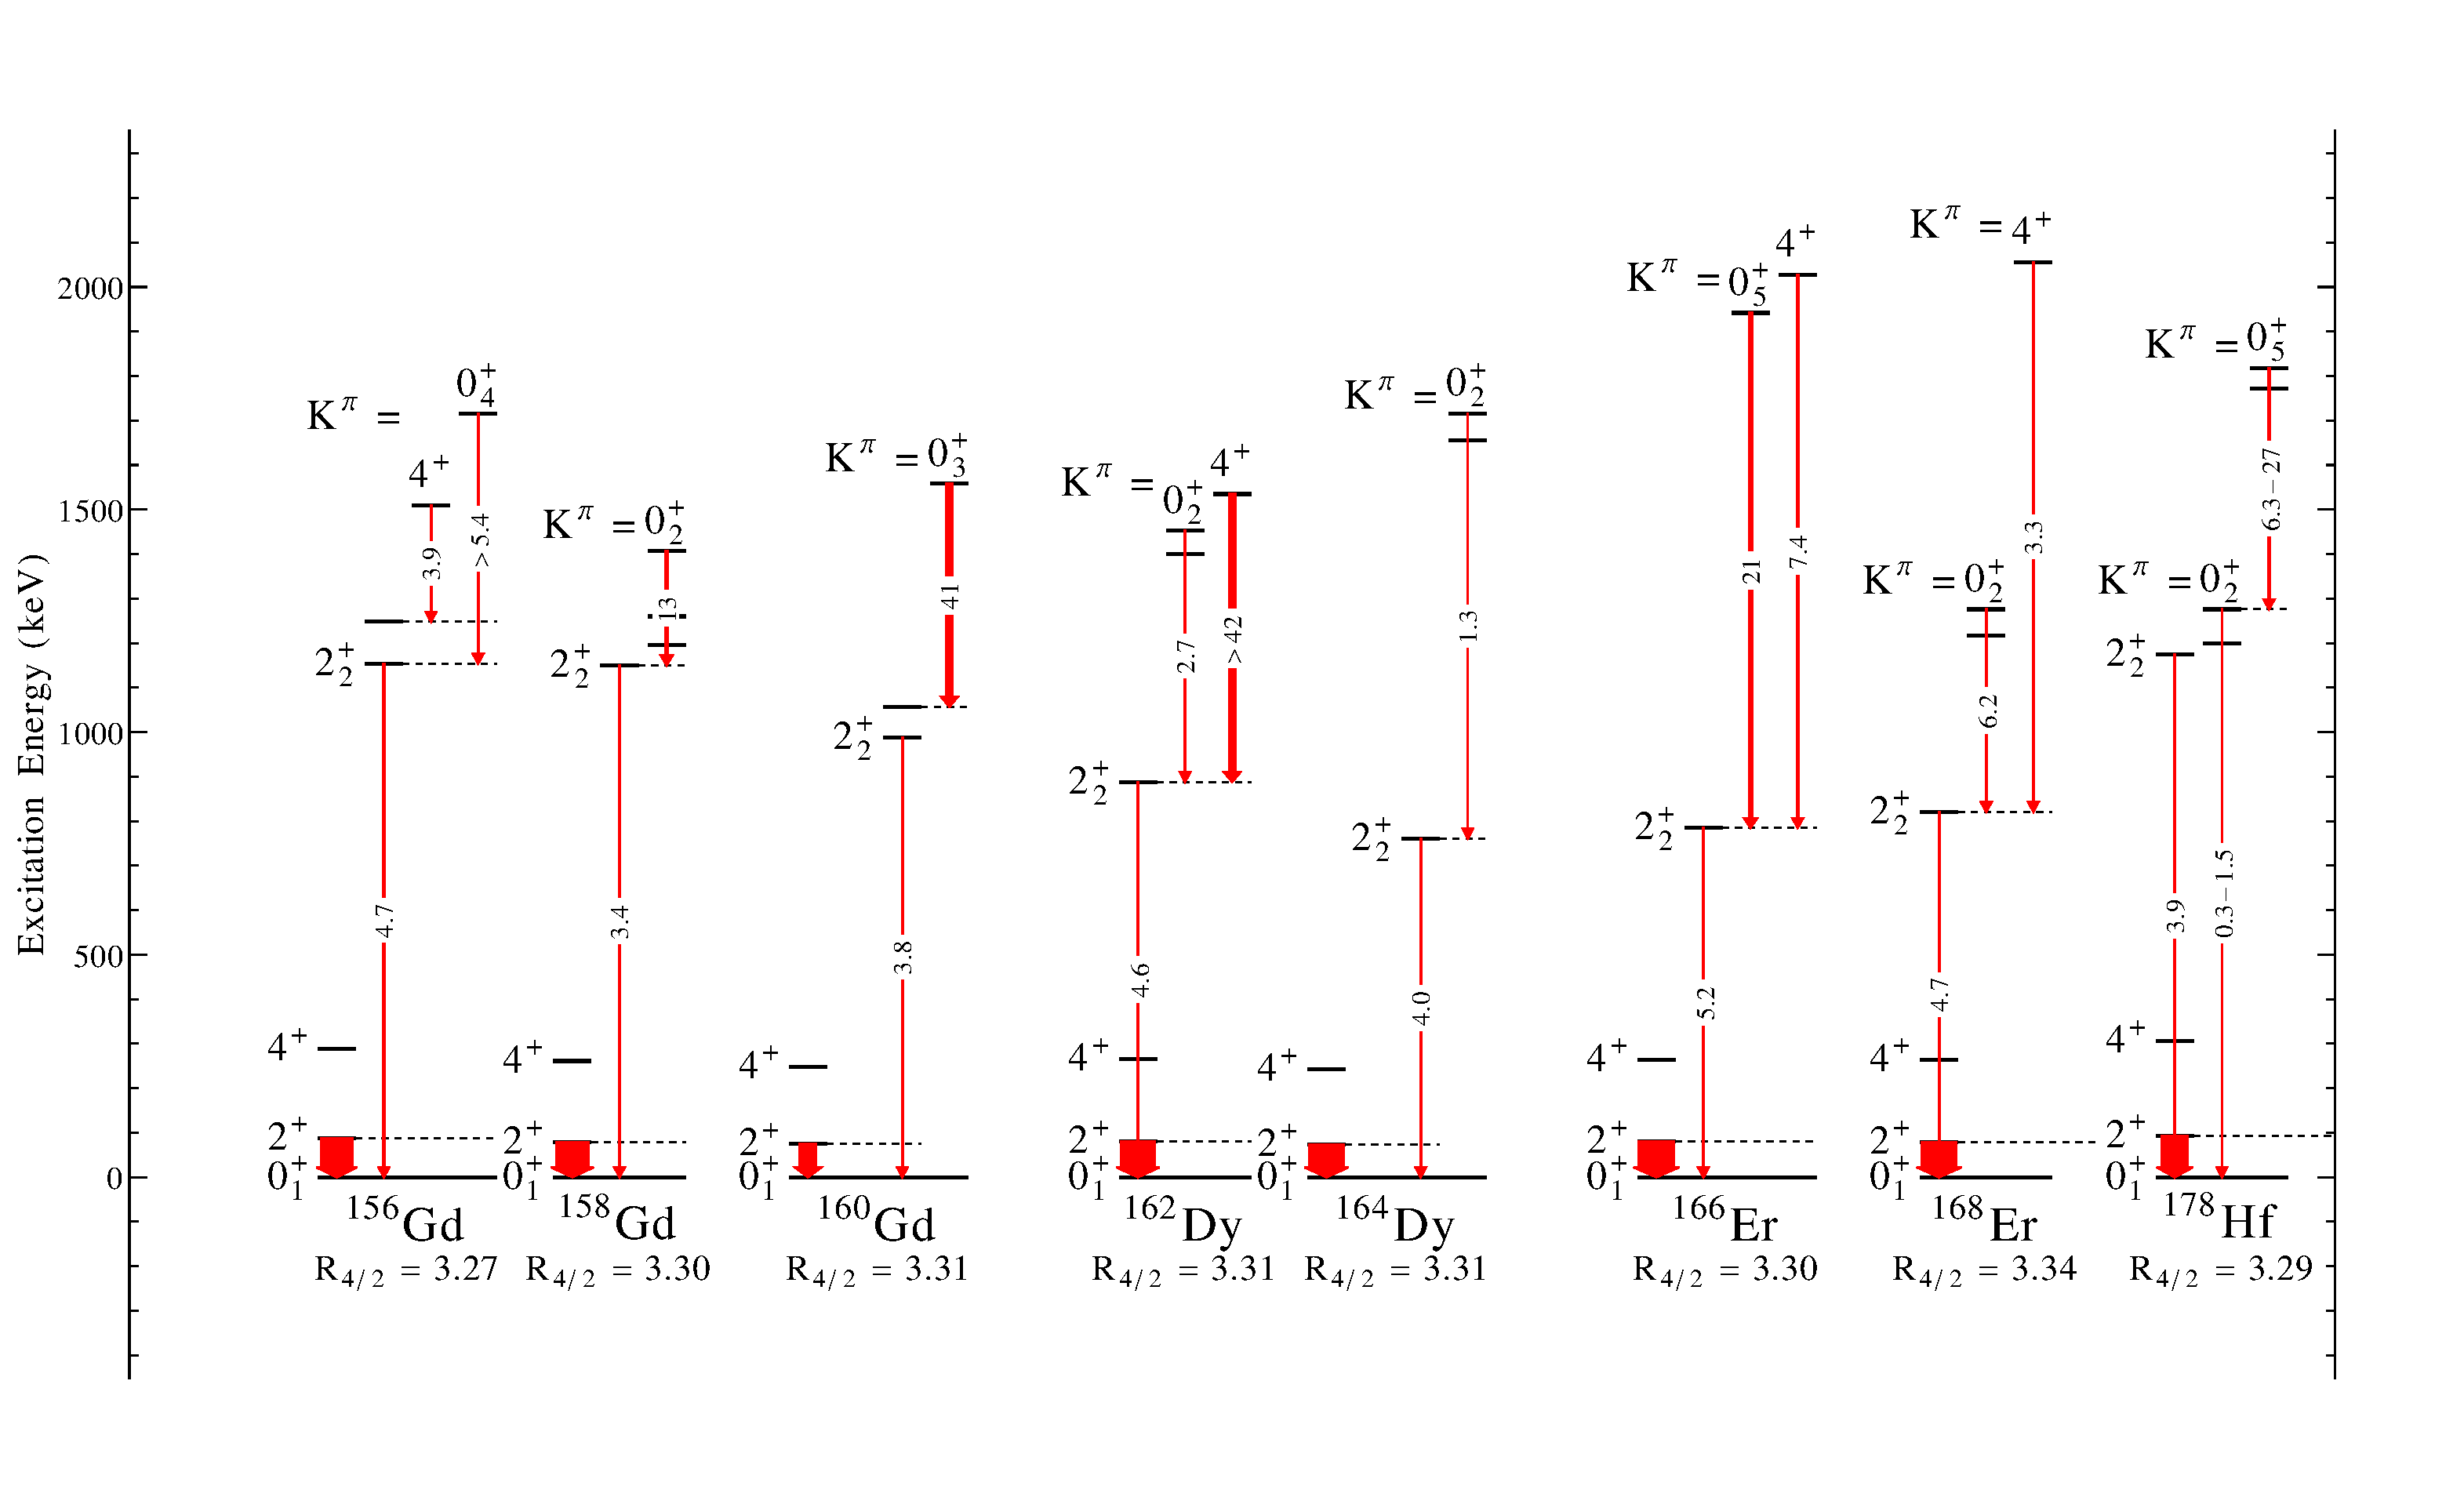
\includegraphics[height=0.8\textheight]{Multiphonon_RareEarths.pdf}
\caption{Summary of all known multiphonon ($\gamma\gamma$, $\beta\gamma$, or $\beta\beta$) configurations in rare-earth nuclei, absolute B(E2) from literature are shown in Weisskopf units to signify collective decays to $\gamma$-vibrational and/or potential $\beta$-vibrational states.
\label{fig:RareEarth_Multiphonon}}
\end{center}
\end{figure}
\end{landscape}

Furthermore, we stress that this problem in nuclear structure is very open, with varied systematic behavior of all K=0 bands in deformed nuclei. In some cases, a collective $\beta$ vibration can be found as the lowest-lying 0$^+$ state, or at a higher excitation energy, in others, the lowest-lying 0$^+$ acts like a collective two-phonon vibration built on top of the $\gamma$-vibration, and in others, one of the higher excitations acts as a $\gamma\gamma$-vibration. Surely, the issue at hand of the nature of 0$^+$ excitations is a wide-open question in nuclear structure, and has been for decades, with a multitude of questions to answer. Can the deformed nucleus act as a near-infinite quantum system with all vibrational degrees available and afforded to it? If we observe well-behaved vibrations in the form of the $\gamma$ bands as the lowest 2$^+$ bands, why do we not have the same B(E2) systematics of the $\beta$-vibration as the lowest 0$^+$ bands? Is the $\beta$ vibration even viable for well-deformed nuclei; if not, what is happening to the $\beta$ vibration across chains of nuclei in the rare-earth region? 


Gadolinium-160 and Dysprosium-162 nuclei both have a very well-deformed shape (R$_\frac{4}{2}$=3.31) as well as a modest number of confirmed and tentative 0$^+$ excitations to study the fasability of vibrational degrees of freedom superimposed on top of a rotational ground state. Literature lifetimes for most states (especially 0$^+$ states and the negative parity states of interest for any octupole correlations) in these nuclei are also scarce, further motivating the lifetime measurements. A great deal of effort and importance is placed on the evolution of nuclear structure across isotopic changes, or at least in a regional scale on the chart of nuclides; the emergence of nuclear data aids in the simultaneous evolution of theoretical efforst to explain the various nuclear structure phenomena at the forefront of nuclear physics. In order to fully ascertain the nature of low-lying excitations (whether they are macroscopic, collective vibrations superimposed on top of a deformed ground state, multiconfigurative particle-quasiparticle states, or something completely different), consistent, precise, and accurate lifetime measurements of excited states must be performed in nuclei where we already have a wealth of spectroscopic knowledge to aid in the characterization of states. 

